\section{الأدوار}
\label{sec:settings-feature-roles}

الدور مجموعة صلاحيات تحمل اسماً، وهو يحدد ما يستطيع حامله رؤيته وفعله. فبدل ضبط الصلاحيات لكل عضو على حدة، تجهّز الدور مرة واحدة ثم تسنده إلى أعضاء أو مناصب أو وحدات تنظيمية، وإذا تغيرت المسؤولية عدّلت الدور في مكان واحد. افتح هذه الصفحة عند ظهور مسؤولية جديدة، أو عندما يرى موظف ما لا يخصه أو لا يجد ما يحتاج إليه. يرى الصفحة من يملك صلاحية عرض الأدوار، أما فتح الدور وإنشاؤه وتعديله وحذفه فلكل منها صلاحية مستقلة.

\begin{rcnote}[مثال: شركة الأفق]
يضغط مسؤول النظام في شركة الأفق ① وينشئ دوراً باسم «منسق الزيارات»، ثم يسنده إلى منصب منسق عمليات. فتصل صلاحياته إلى عمر حداد لأنه يشغل هذا المنصب، ولا تصل إلى سارة الخطيب.
\end{rcnote}

\begin{figure}[H]
\centering
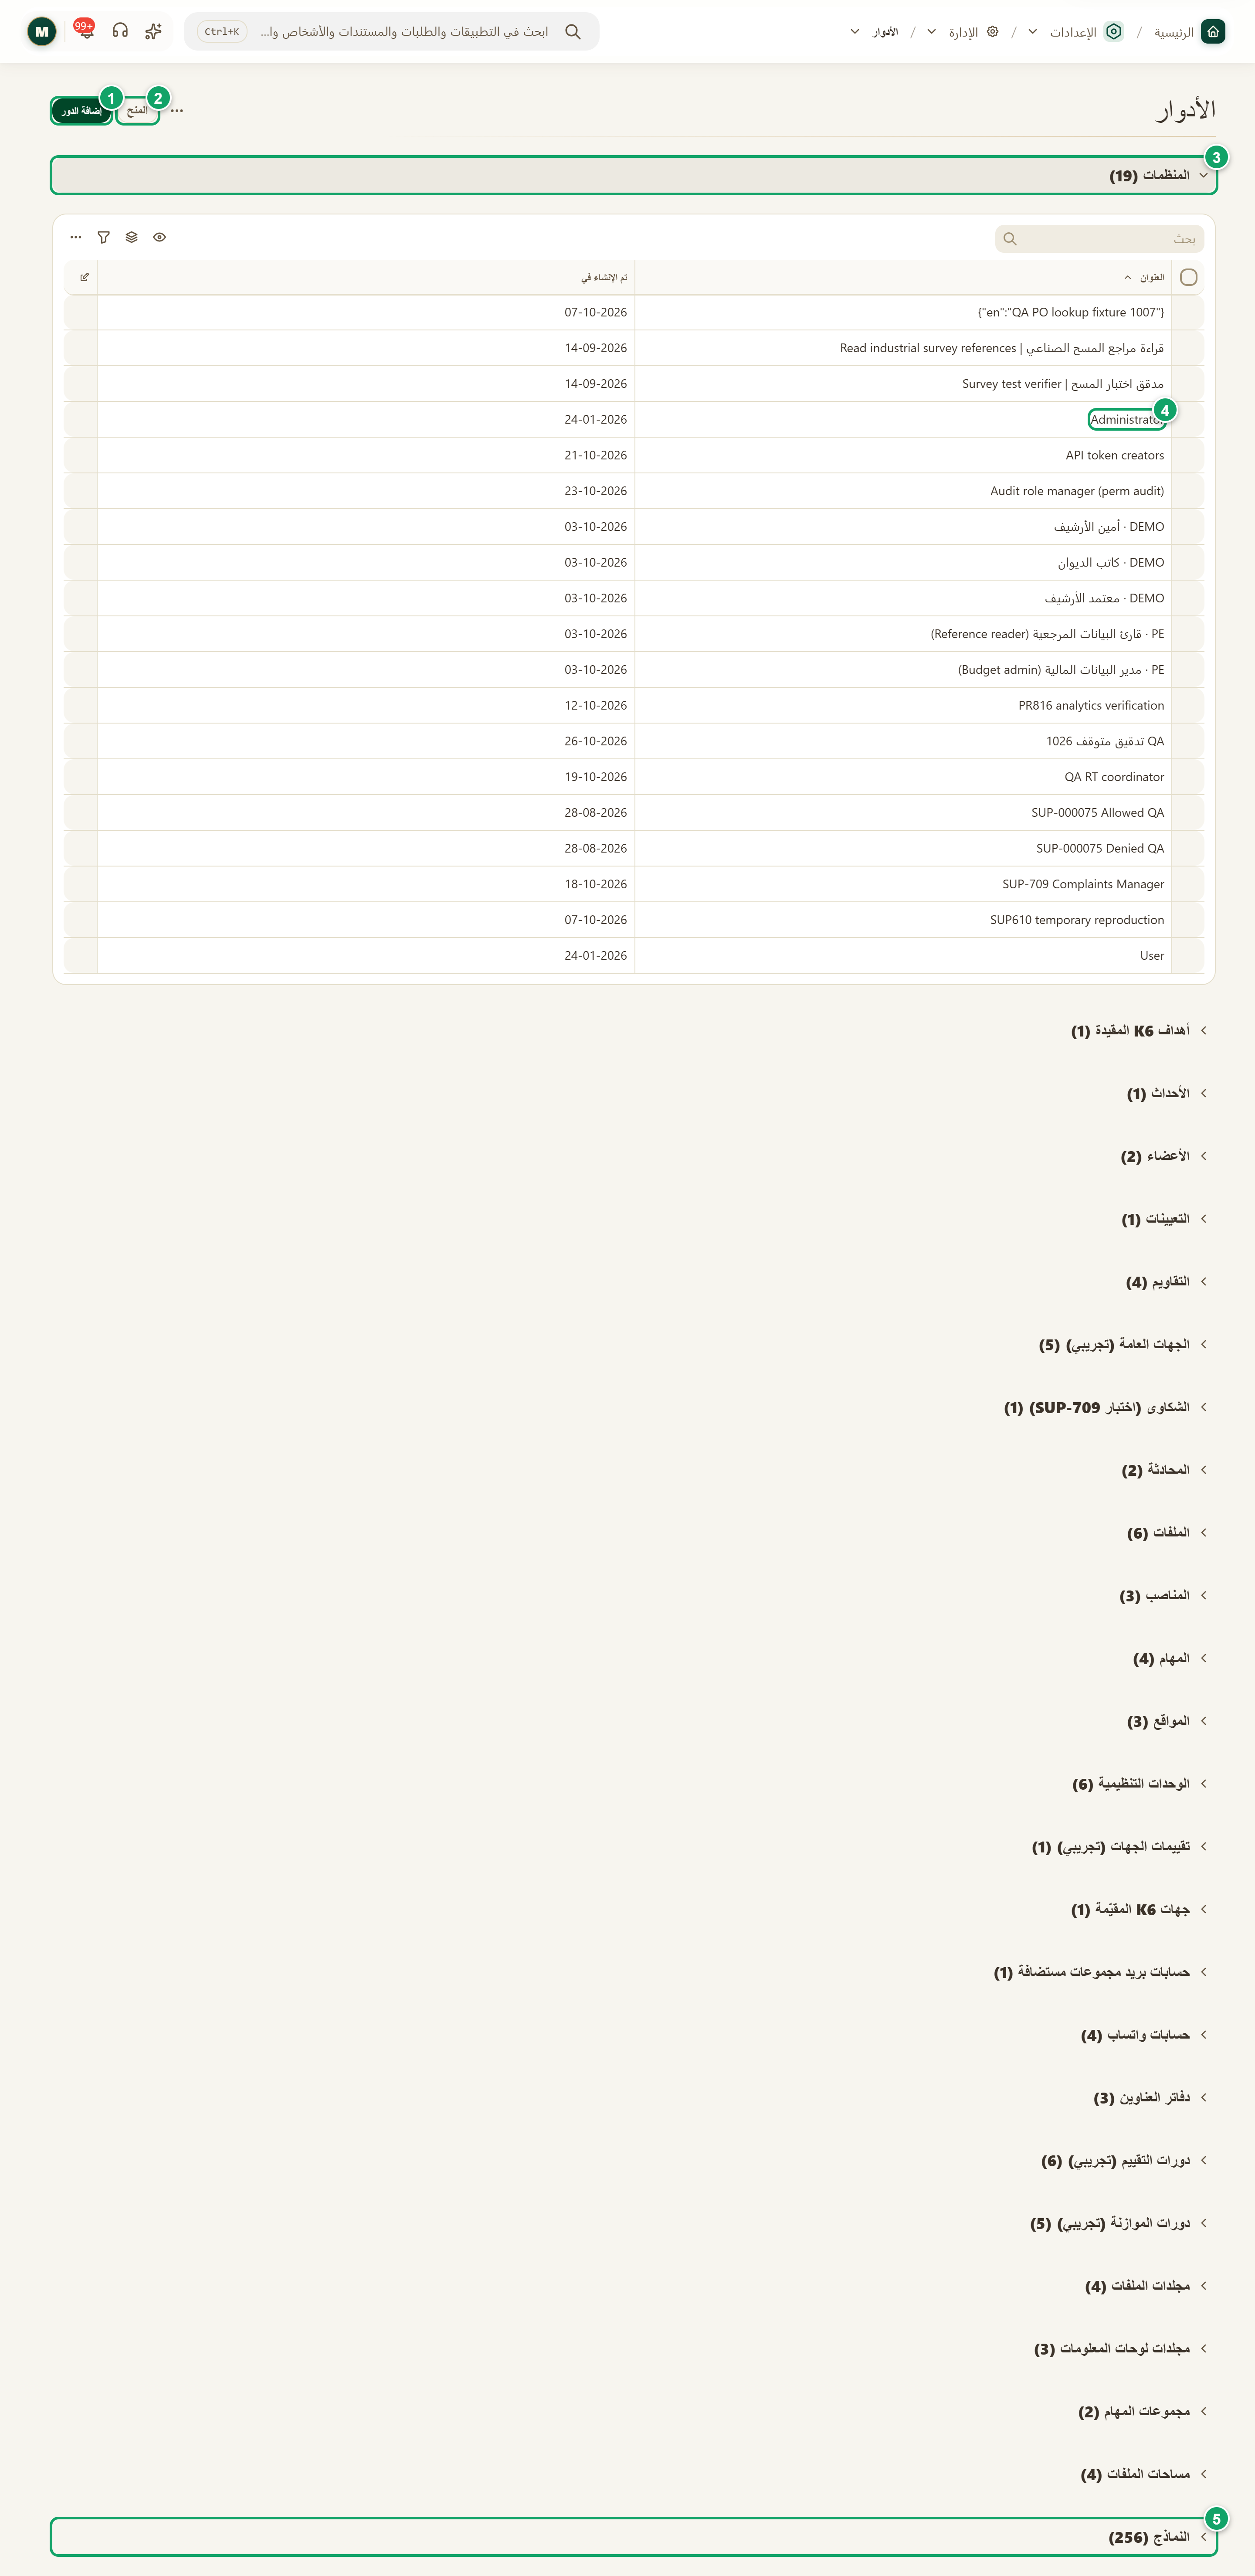
\includegraphics[width=0.95\linewidth,height=0.72\textheight,keepaspectratio]{figures/screens/ch08-roles-ar.png}
\caption{قائمة الأدوار مجمّعة بحسب النطاق}
\label{fig:settings-roles-screen}
\shotnote{تعرض الصفحة الأدوار في مجموعات بحسب النطاق، والنطاق هو المكان الذي تسري فيه صلاحيات الدور: المؤسسة كلها، أو نوع سجل معين، أو نموذج واحد. ويبين الرقم بجانب كل مجموعة عدد أدوارها، فاضغط اسم المجموعة لفتحها. ① «إضافة الدور». ② «المنح»: قواعد من يحق له إسناد الأدوار. ③ مجموعة الأدوار التي تسري على المؤسسة كلها. ④ صف الدور: اضغطه لفتح الدور؛ وتجد في قائمة الصف أمر «نسخ». ⑤ «النماذج»: أدوار خاصة بنموذج واحد، مجمّعة تحت اسمه.}
\end{figure}

\begin{figure}[H]
\centering
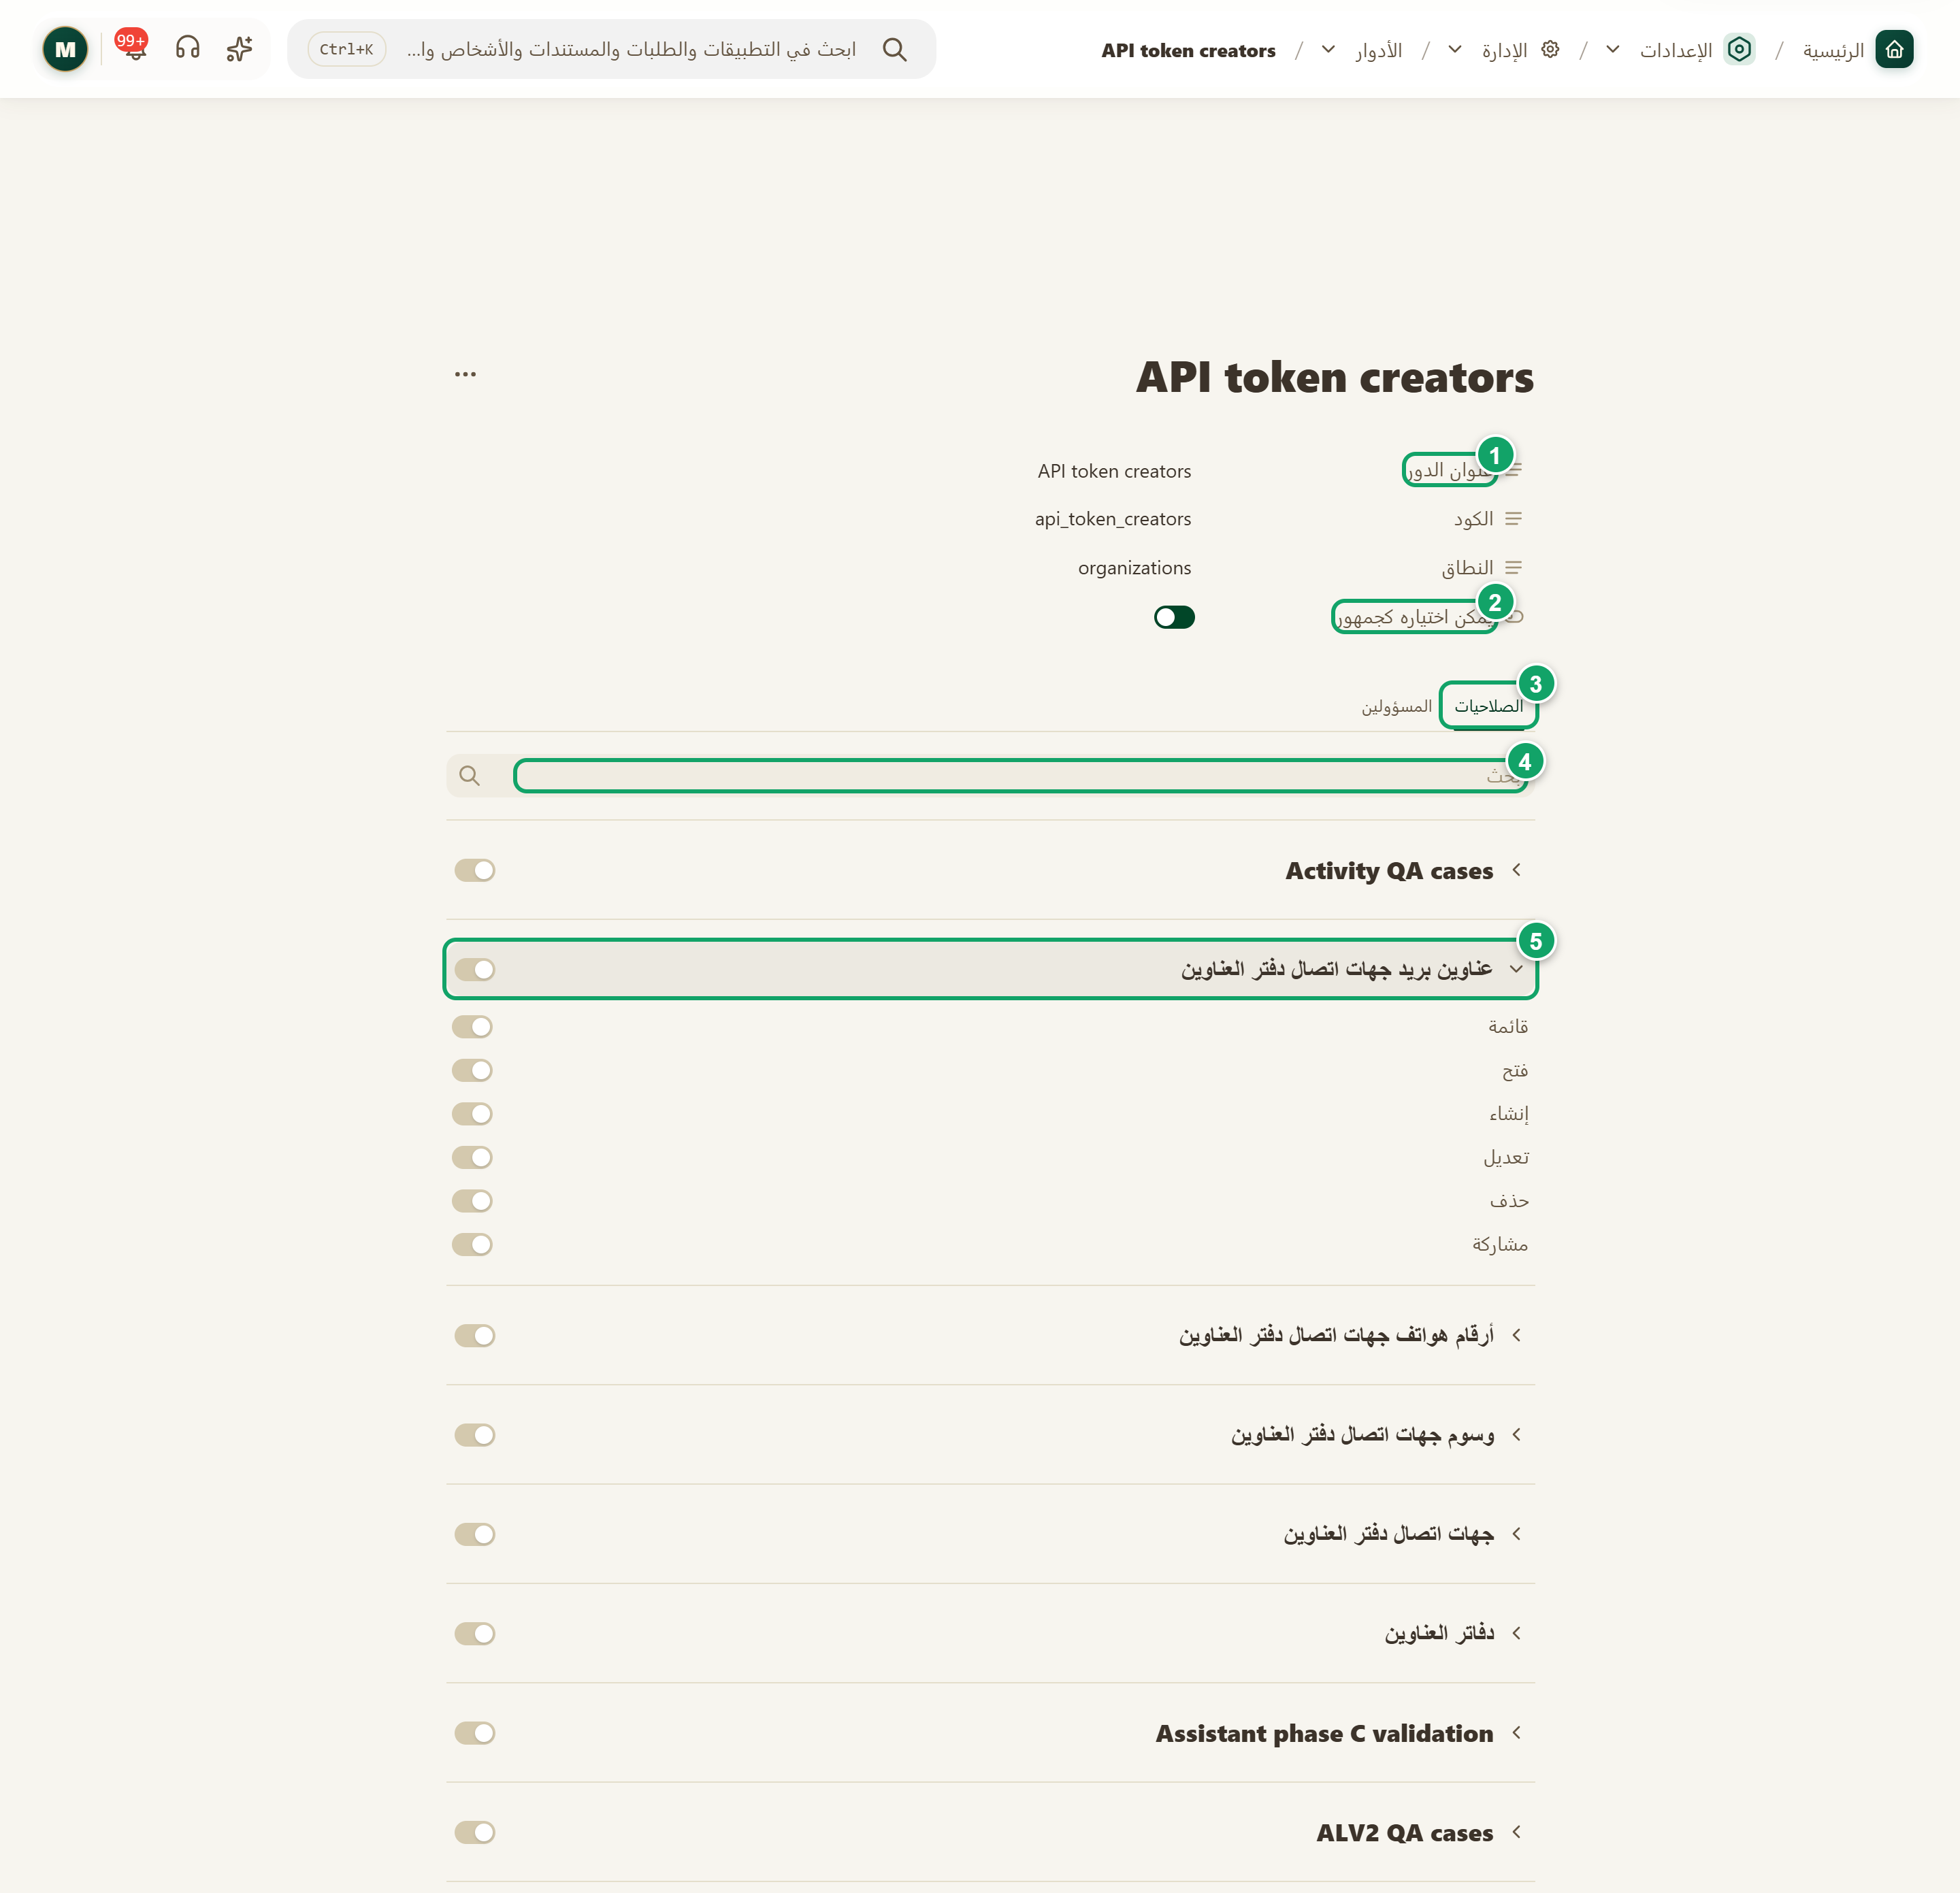
\includegraphics[width=0.95\linewidth,height=0.72\textheight,keepaspectratio]{figures/screens/ch08-roles-permissions-ar.png}
\caption{صفحة الدور: تبويب «الصلاحيات»}
\label{fig:settings-roles-permissions-screen}
\shotnote{يضم هذا التبويب كل أنواع السجلات التي يمكن أن يشملها الدور، ويفتح كل صف على مفاتيح منفصلة مثل العرض والفتح والإنشاء والتعديل. والدور المعروض دور اختباري فُتح للقراءة فقط. ① «عنوان الدور». ② «يمكن اختياره كجمهور»: يتيح لأدوات المشاركة والإسناد اختيار حاملي هذا الدور، ويُحفظ فور تغييره. ③ «الصلاحيات». ④ حقل البحث: يختصر القائمة الطويلة. ⑤ صف نوع السجل: اضغط اسمه لفتحه، ويفعّل المفتاح في طرفه كل صلاحياته معاً.}
\end{figure}

\begin{figure}[H]
\centering
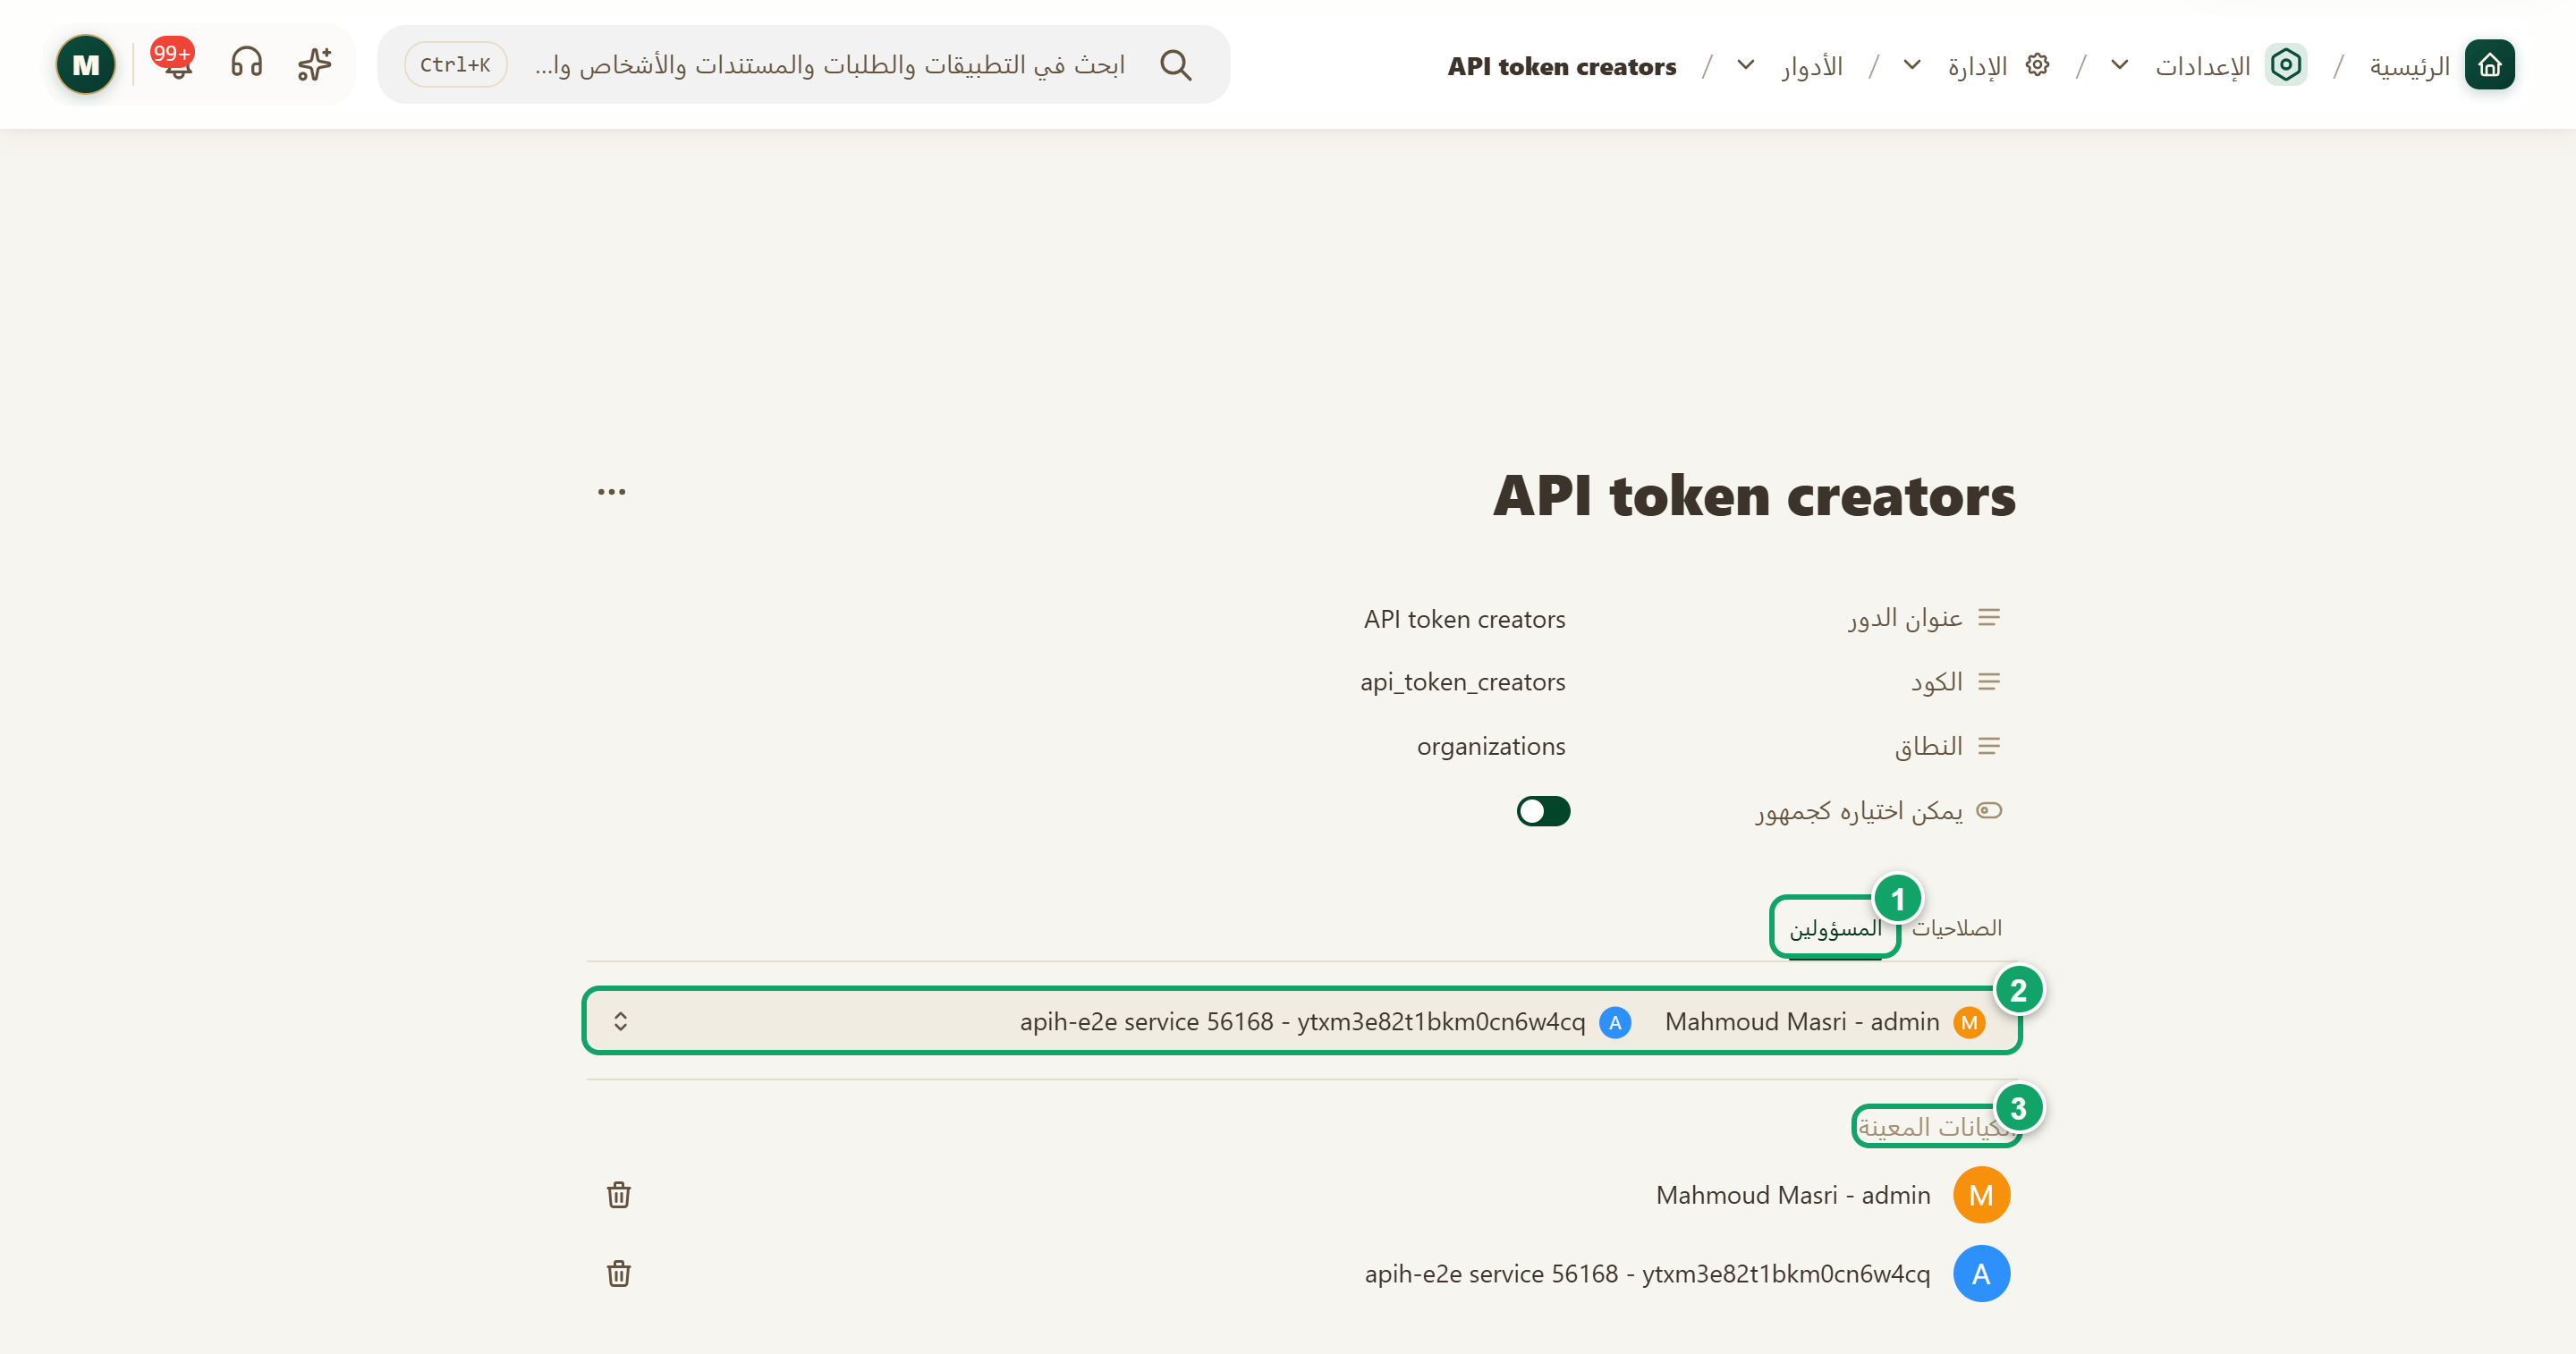
\includegraphics[width=0.95\linewidth,height=0.72\textheight,keepaspectratio]{figures/screens/ch08-roles-assignees-ar.png}
\caption{صفحة الدور: تبويب «المسؤولين»}
\label{fig:settings-roles-assignees-screen}
\shotnote{لا يعمل الدور إلا إذا أُسند إلى أحد، وهذا التبويب هو مكان الإسناد. وتُكتب تغييرات هذا التبويب مباشرة، أما تغييرات الصلاحيات فتنتظر زر «حفظ». ① «المسؤولين». ② حقل الإسناد: اختر منه عضواً أو منصباً أو وحدة تنظيمية. ③ «الكيانات المعينة»: من يحمل الدور الآن، ويزيل زر الحذف بجانب الاسم الإسناد.}
\end{figure}

\begin{table}[H]
\centering
\caption{ماذا تسجل في الدور؟}
\label{tab:settings-roles-fields}
\begin{tabularx}{\linewidth}{R{4.2cm} Y}
\rcHeaderRow
\thh{الحقل} & \thh{ما الذي تسجله فيه؟}\\
«عنوان الدور» \req & اسم يصف المسؤولية، ويمكن تغييره لاحقاً.\\
«الكود» \opt & معرّف الدور. إذا تركته فارغاً ولّده النظام من العنوان، ولا يتغير بعد الإنشاء.\\
«النطاق» & «المنظمات» للمؤسسة كلها، أو نوع سجل يسمح بذلك، أو نموذج محدد. لا يتغير بعد الإنشاء.\\
«يمكن اختياره كجمهور» & يكون مفعّلاً في الدور الجديد. عطّله إذا أردت ألا تعرض أدوات المشاركة والإسناد هذا الدور.\\
«تعيين للمُنشئ» & يظهر في أدوار نوع السجل والنموذج، ويمنح منشئ العنصر هذا الدور عليه تلقائياً.\\
«المحدد» & يظهر عندما يكون لنوع السجل تسلسل هرمي، ويحدد هل يسري الدور على العنصر نفسه أو على ما فوقه أو ما تحته.\\
«الصلاحيات» & المفاتيح المسموح بها لكل نوع سجل. وفي الأدوار المرتبطة بوحدة أو موقع أو منصب قد يظهر خيار «السجلات» لقصرها على قيمة واحدة من حقل.\\
«المسؤولين» & الأعضاء والمناصب والوحدات التنظيمية التي تحمل الدور.\\
\end{tabularx}
\end{table}

\begin{figure}[H]
\centering
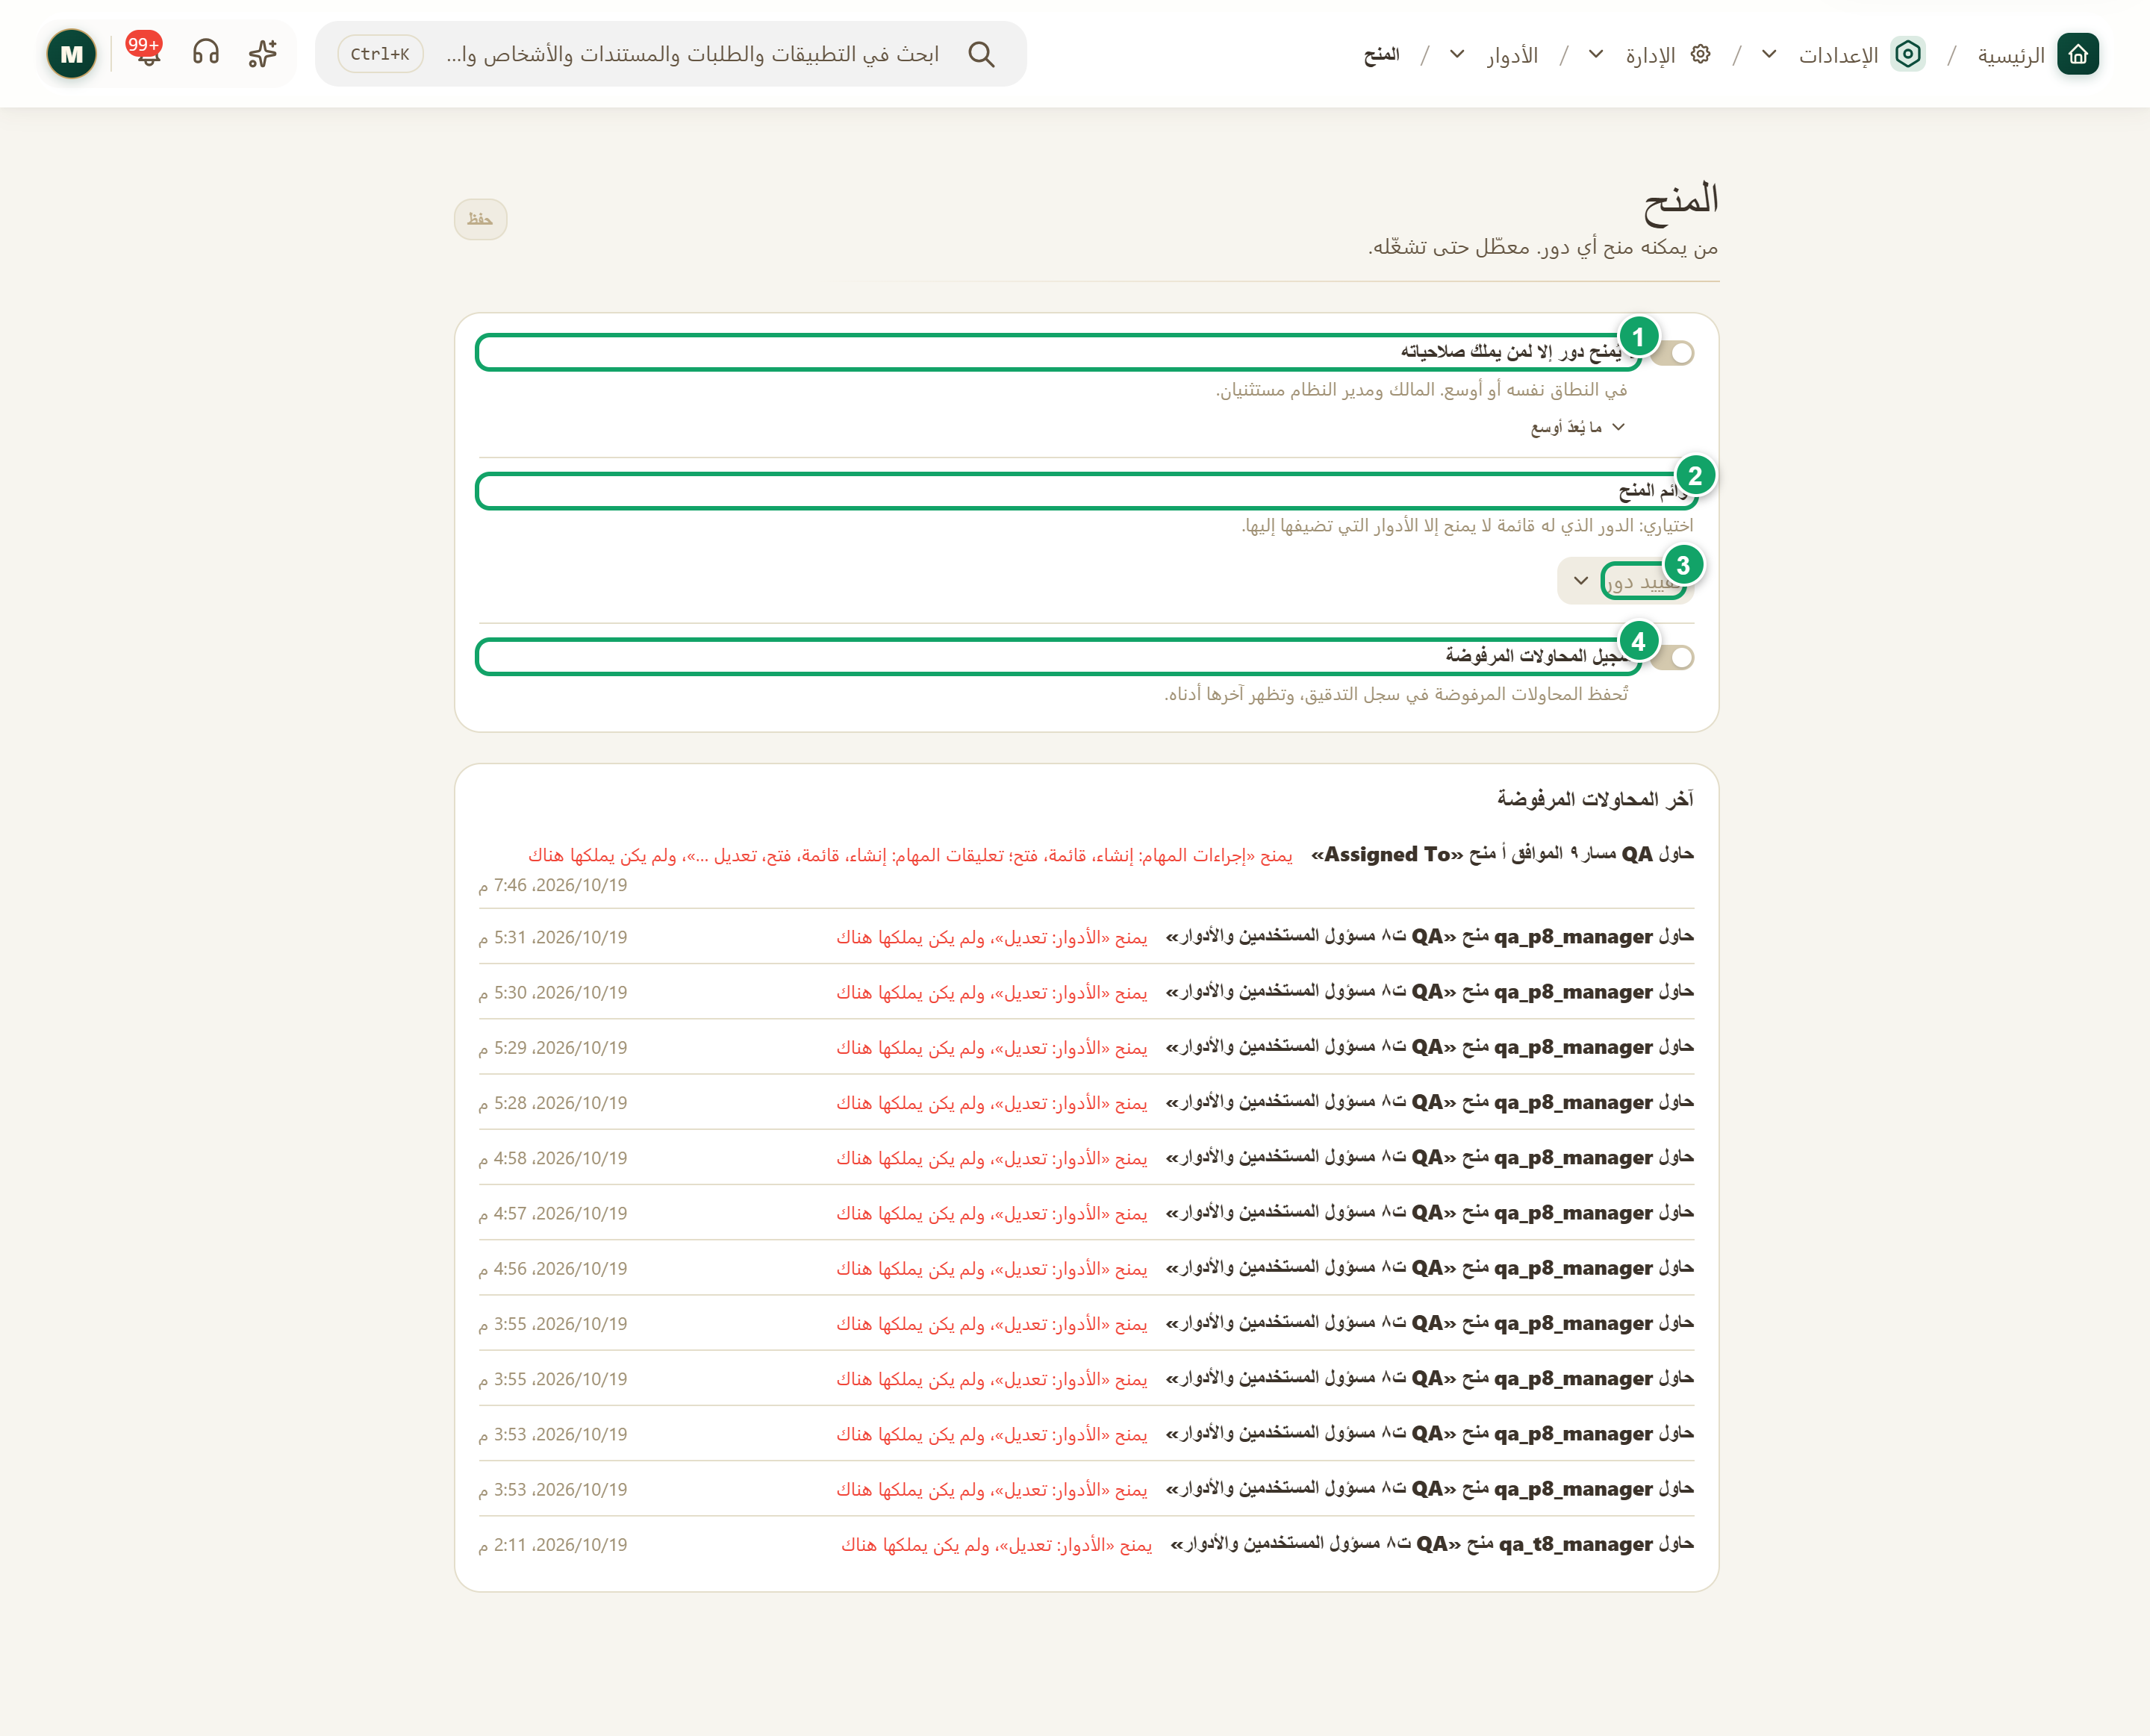
\includegraphics[width=0.95\linewidth,height=0.72\textheight,keepaspectratio]{figures/screens/ch08-roles-grants-ar.png}
\caption{صفحة «المنح»}
\label{fig:settings-roles-grants-screen}
\shotnote{تضبط هذه الصفحة من يستطيع إسناد الأدوار، لا ما تمنحه الأدوار نفسها. وهي معطّلة حتى تشغّلها، والقائمة السفلية في الصورة محاولات اختبارية مرفوضة. ① المفتاح الرئيسي: يمنع إسناد دور يحمل صلاحيات لا يملكها المُسنِد في النطاق نفسه أو نطاق أوسع، ويُستثنى المالك وحاملو دور المسؤول. ② «قوائم المنح». ③ «تقييد دور»: يحصر ما يمنحه حامل دور معين في أدوار تختارها. ④ «تسجيل المحاولات المرفوضة».}
\end{figure}

\begin{enumerate}
\item اضغط «إضافة الدور»، واكتب «عنوان الدور»، واختر «النطاق»، ثم اضغط «إنشاء الدور». يفتح النظام صفحة الدور الجديد.
\item في «الصلاحيات»، ابحث عن نوع السجل واضغط اسمه، ثم فعّل ما يلزم فقط. يفعّل النظام ما تعتمد عليه الصلاحية تلقائياً؛ فتشغيل «فتح» يشغّل معه «قائمة».
\item اضغط «حفظ» في شريط «تغييرات غير محفوظة».
\item افتح «المسؤولين» وأضف الأعضاء أو المناصب أو الوحدات.
\item لتشخيص مشكلة وصول، افتح قائمة النقاط الثلاث بجانب «المنح» واختر «تصحيح أدوار المستخدم» أو «شرح الصلاحية».
\item لحذف دور، افتحه واضغط النقاط الثلاث بجانب عنوانه، ثم اختر «حذف الدور» وأكّد. لا يمكن التراجع عن الحذف، ولا يُحذف الدور المقفل.
\end{enumerate}

\textbf{تحقق:} أعد فتح الدور وتأكد من بقاء المفاتيح مفعّلة، ومن ظهور الاسم الصحيح في «الكيانات المعينة». ثم اطلب من عضو يحمل الدور تجربة العمل المطلوب وعملاً آخر يجب أن يبقى ممنوعاً؛ فقد يمنحه دور آخر الصلاحية نفسها.

\clearpage
\section{التحقق بخطوتين}
\label{sec:settings-feature-two-step}

يضيف التحقق بخطوتين إثباتاً ثانياً بعد كلمة المرور، فلا تكفي كلمة مرور مسروقة لدخول الحساب. والخطوة الثانية إما رمز يتغير كل 30 ثانية في تطبيق مصادقة على الهاتف، وإما مفتاح مرور محفوظ على جهاز العضو ويُحتسب خطوة ثانية بمفرده. من هذه الصفحة تقرر من يلزمه ذلك، وتتابع من أتم الإعداد. لا يفتحها إلا مالك المؤسسة ومن يحمل دور المسؤول، وتمس إعداداتها تسجيل دخول الأعضاء؛ فأبلغهم قبل تغييرها.

\begin{rcnote}[مثال: شركة الأفق]
يختار مسؤول النظام في شركة الأفق «المسؤولون» عند ①، ويترك عند ② فترة سماح مدتها 14 يوماً، فيبدأ بحماية الحسابات الأوسع صلاحية. ثم يراجع النسبة عند ⑤ قبل أن يوسّع الاشتراط ليشمل سارة الخطيب وعمر حداد.
\end{rcnote}

\begin{figure}[H]
\centering
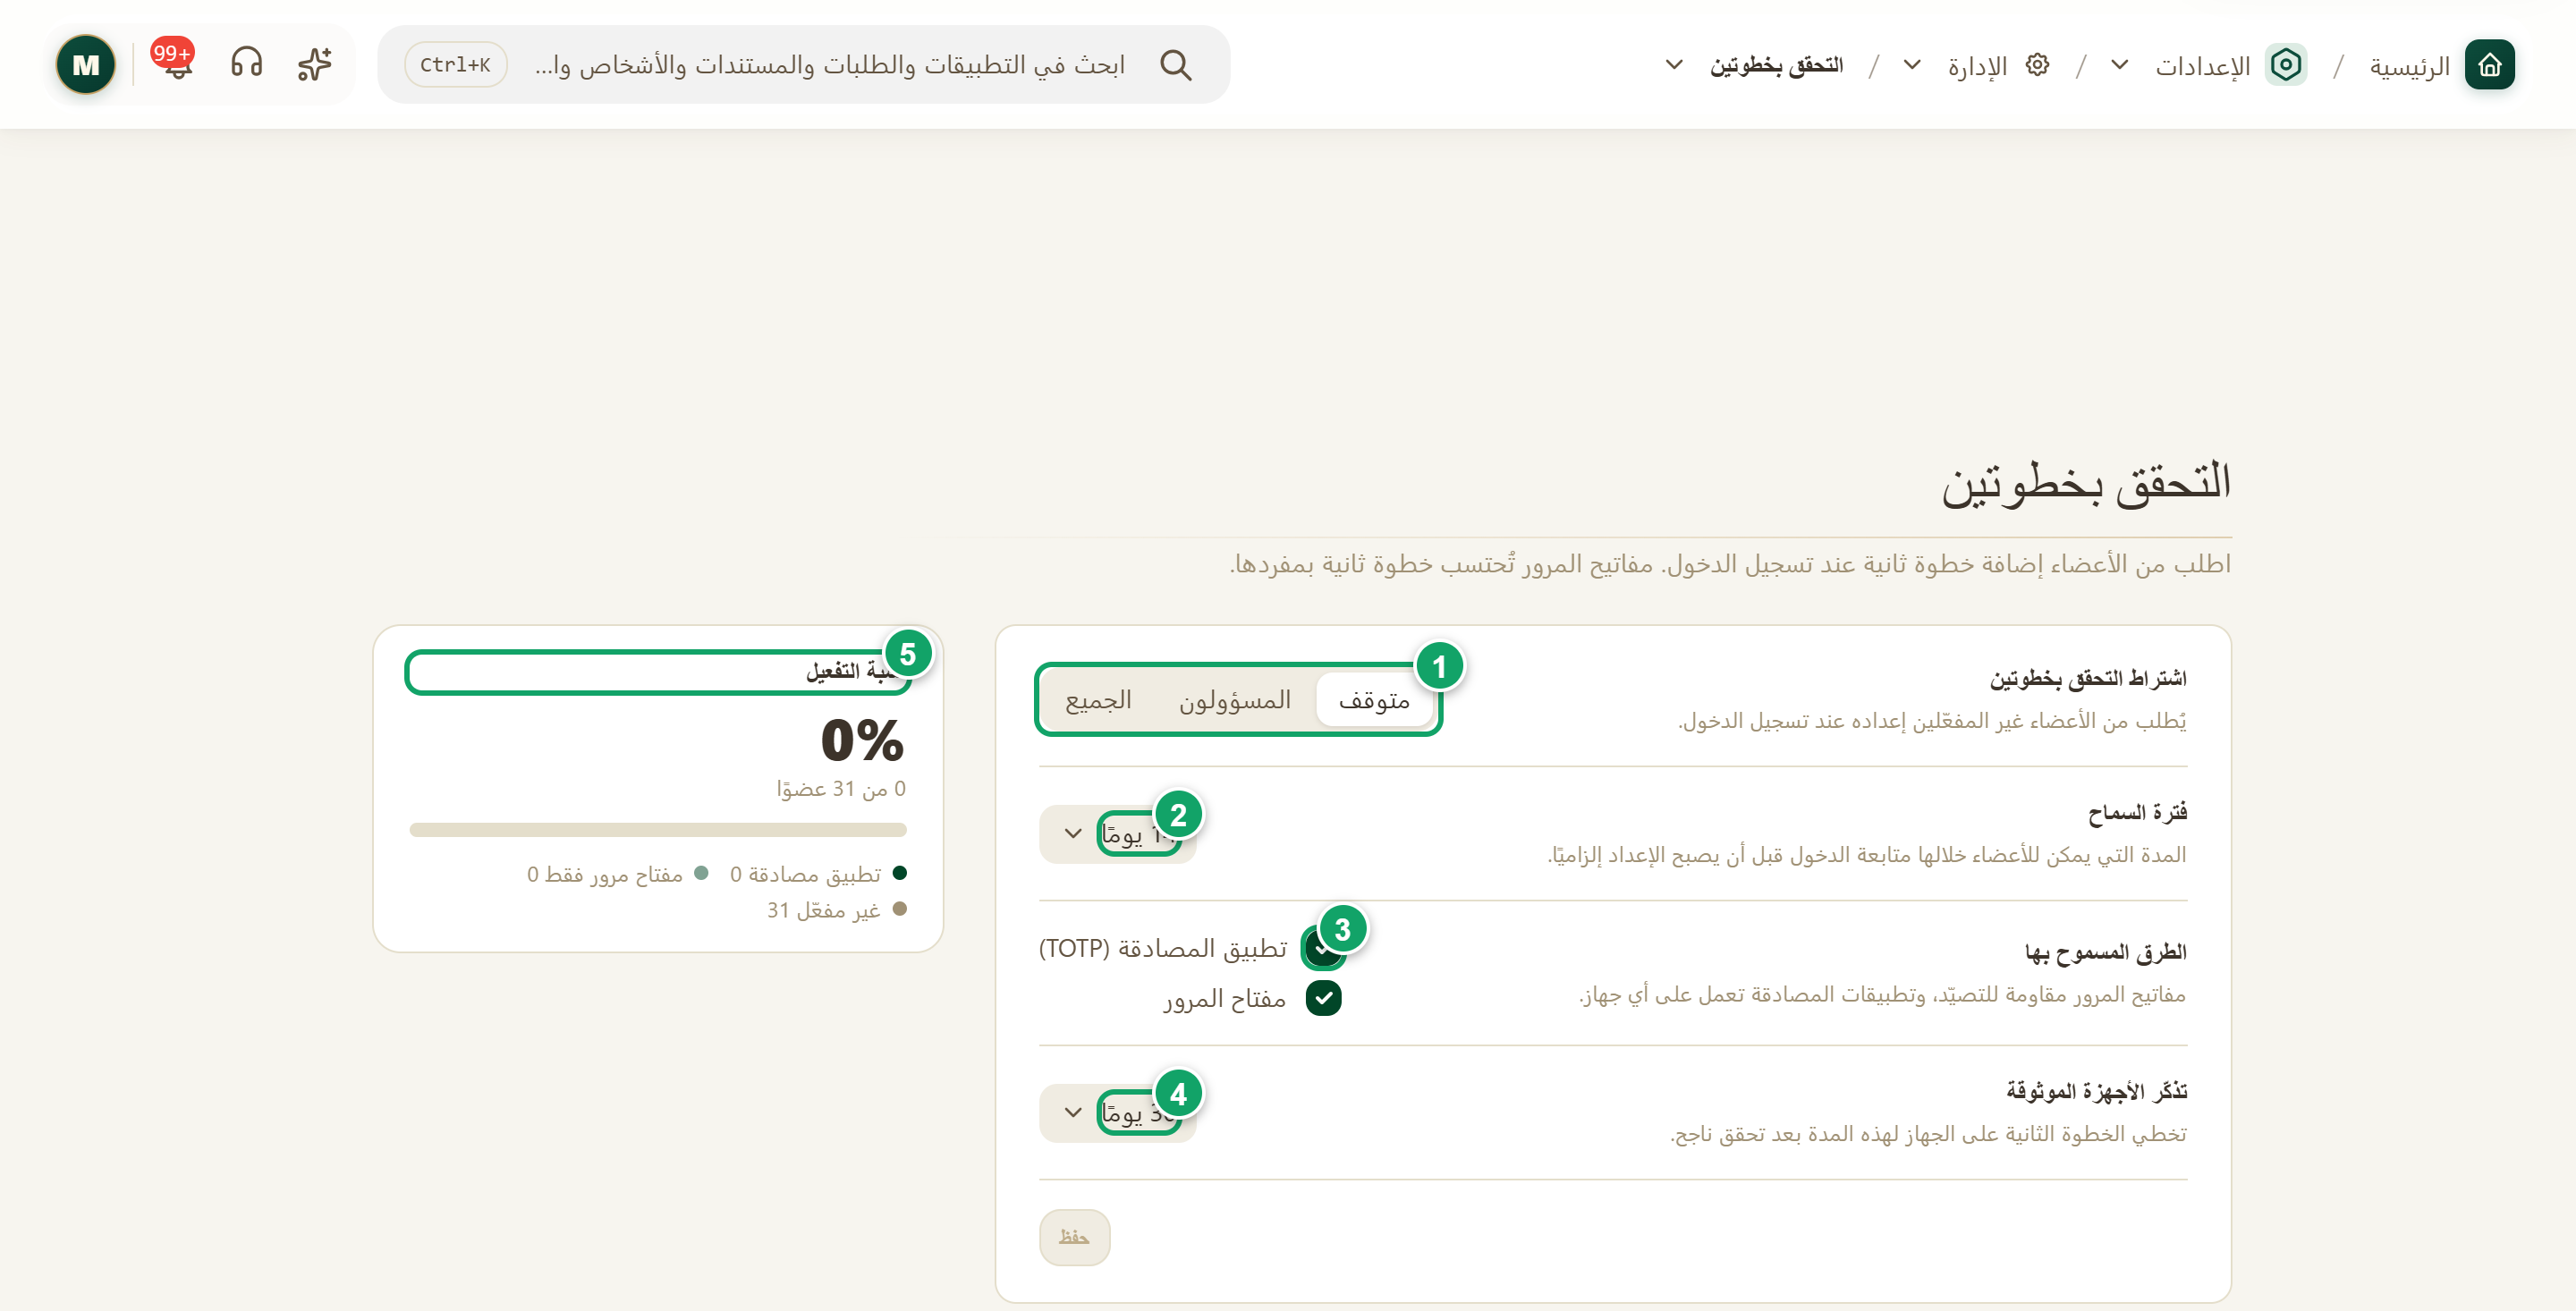
\includegraphics[width=0.95\linewidth,height=0.72\textheight,keepaspectratio]{figures/screens/ch08-two-step-ar.png}
\caption{سياسة التحقق بخطوتين ونسبة التفعيل}
\label{fig:settings-two-step-screen}
\shotnote{تجمع الصفحة قرار المؤسسة ونتيجته: الإعدادات في البطاقة الكبيرة، وعدد من فعّلوا الخطوة الثانية في البطاقة الجانبية. والاشتراط متوقف في بيئة الاختبار، لذلك لا تظهر قائمة الأعضاء المتأخرين. ① «اشتراط التحقق بخطوتين». ② «فترة السماح». ③ «الطرق المسموح بها»: يجب أن تبقى طريقة واحدة على الأقل. ④ «تذكّر الأجهزة الموثوقة». ⑤ «نسبة التفعيل»: تظهر تحتها قائمة «لم يُفعَّل بعد» عند تشغيل الاشتراط.}
\end{figure}

\begin{table}[H]
\centering
\caption{ماذا تسجل في سياسة التحقق بخطوتين؟}
\label{tab:settings-two-step-fields}
\begin{tabularx}{\linewidth}{R{4.2cm} Y}
\rcHeaderRow
\thh{الحقل} & \thh{ما الذي تسجله فيه؟}\\
«اشتراط التحقق بخطوتين» & «متوقف»، أو «المسؤولون» وهم المالك وحاملو دور المسؤول، أو «الجميع».\\
«فترة السماح» & «بلا فترة» أو 7 أو 14 أو 30 يوماً. تُحسب من يوم تشغيل الاشتراط، أو من تاريخ إضافة العضو إذا انضم بعده.\\
«الطرق المسموح بها» & «تطبيق المصادقة (\en{TOTP})» و«مفتاح المرور». لا يمكن إلغاء الطريقتين معاً.\\
«تذكّر الأجهزة الموثوقة» & «أبدًا» أو 7 أو 30 أو 90 يوماً، وهي مدة تخطي الخطوة الثانية على الجهاز بعد تحقق ناجح.\\
\end{tabularx}
\end{table}

\begin{enumerate}
\item اختر من يشمله الاشتراط، ثم اختر «فترة السماح» و«الطرق المسموح بها» و«تذكّر الأجهزة الموثوقة».
\item اضغط «حفظ». قبل الحفظ يعيد «تجاهل» الصفحة إلى آخر إعدادات محفوظة.
\item تابع قائمة «لم يُفعَّل بعد»، واضغط «إرسال تذكير» بجانب العضو أو زر التذكير الجماعي تحت القائمة.
\item إذا فقد عضو هاتفه، فافتح سجله وتبويب «التحقق بخطوتين»، ثم اكتب السبب واضغط «إعادة تعيين التحقق بخطوتين». يحتاج ذلك إلى صلاحية إعادة تعيين كلمة مرور العضو، ويزيل تطبيق المصادقة ورموز الاسترداد ويسجّل خروجه، وتبقى مفاتيح المرور.
\end{enumerate}

\textbf{تحقق:} ترتفع «نسبة التفعيل» كلما أتم عضو الإعداد، ويظهر لمن لم يكمله عدد الأيام المتبقية. عند انتهاء فترة السماح يُطلب من العضو الإعداد قبل إكمال الدخول. أما إذا ألغيت «تطبيق المصادقة (\en{TOTP})» فلا يُفرض الإعداد عند انتهاء فترة السماح على من ليس لديه مفتاح مرور، فأبقِ هذه الطريقة مفعّلة إذا أردت الإلزام.

\clearpage
\section{الجلسات والأجهزة}
\label{sec:settings-feature-sessions}

الجلسة هي المدة التي يبقى فيها العضو مسجّلاً على جهاز دون إعادة كتابة كلمة المرور. كلما طالت كان العمل أسهل، وكلما قصرت قلّ خطر جهاز منسي أو مفقود. تضبط هذه الصفحة تلك الموازنة للمؤسسة كلها: مدة الجلسة لكل نوع جهاز، والخروج بعد عدم النشاط، وعدد الأجهزة، وتنبيهات الأجهزة الجديدة. لا يفتحها إلا مالك المؤسسة ومن يحمل دور المسؤول. وتسري التغييرات على عمليات الدخول الجديدة، لا على الجلسات المفتوحة.

\begin{rcnote}[مثال: شركة الأفق]
يخفض مسؤول النظام في شركة الأفق مدة الويب عند ① لأن بعض موظفي فرع حلب يستخدمون أجهزة مشتركة، ويبقي التنبيهات مفعّلة عند ③. فإذا دخل عمر حداد من جهاز جديد وصله تنبيه، ثم يراجع المسؤول الأثر العام عند ④ قبل الحفظ.
\end{rcnote}

\begin{figure}[H]
\centering
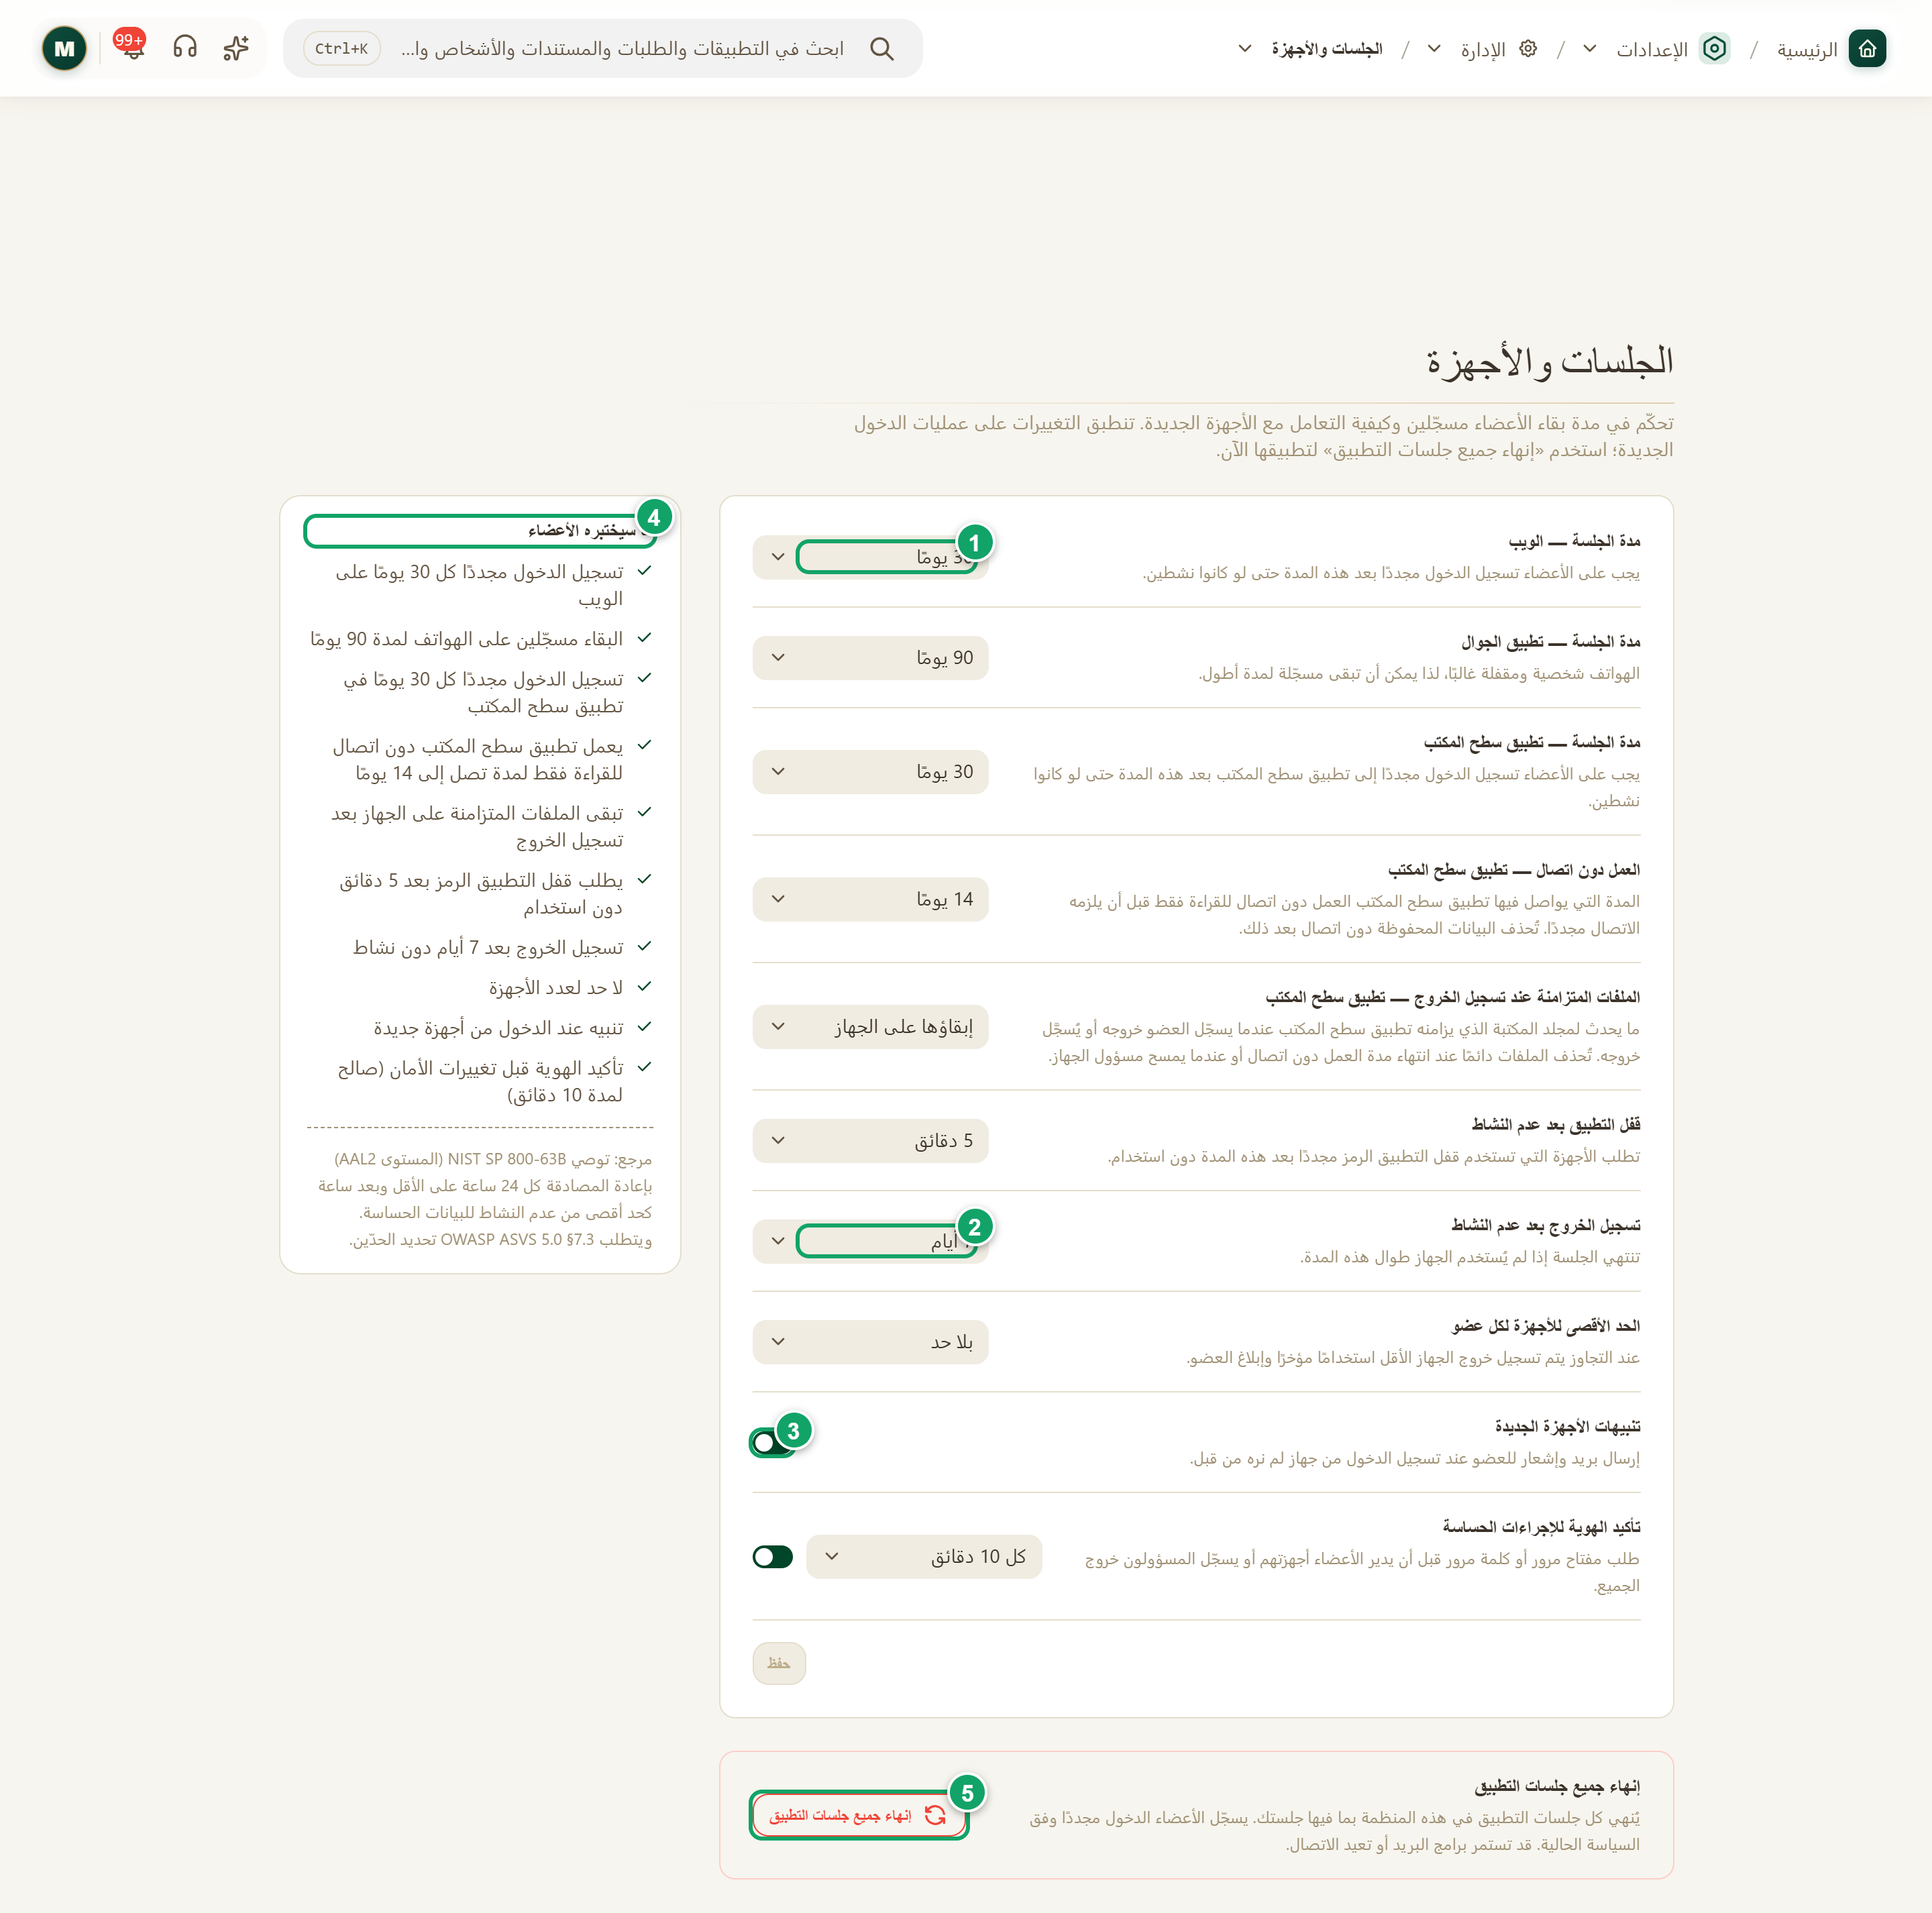
\includegraphics[width=0.95\linewidth,height=0.72\textheight,keepaspectratio]{figures/screens/ch08-sessions-ar.png}
\caption{سياسة الجلسات والأجهزة}
\label{fig:settings-sessions-screen}
\shotnote{تترجم البطاقة الجانبية الإعدادات إلى ما سيلمسه الأعضاء فعلاً، وتتغير مع كل اختيار قبل الحفظ. وتظهر الصفحة هنا بقيمها الحالية في بيئة الاختبار، ولم يُغيَّر فيها شيء. ① «مدة الجلسة — الويب». ② «تسجيل الخروج بعد عدم النشاط». ③ «تنبيهات الأجهزة الجديدة». ④ «ما سيختبره الأعضاء». ⑤ «إنهاء جميع جلسات التطبيق»: يخرج الجميع فوراً، وأنت معهم.}
\end{figure}

\begin{table}[H]
\centering
\caption{ماذا تسجل في سياسة الجلسات؟}
\label{tab:settings-sessions-fields}
\begin{tabularx}{\linewidth}{R{4.2cm} Y}
\rcHeaderRow
\thh{الحقل} & \thh{ما الذي تسجله فيه؟}\\
«مدة الجلسة — الويب» & من 8 ساعات إلى 30 يوماً. يعيد العضو الدخول بعدها حتى لو كان نشطاً.\\
«مدة الجلسة — تطبيق الجوال» & من 7 إلى 180 يوماً.\\
«مدة الجلسة — تطبيق سطح المكتب» & من 8 ساعات إلى 90 يوماً.\\
«العمل دون اتصال — تطبيق سطح المكتب» & من يوم إلى 30 يوماً للقراءة فقط، ثم تُحذف البيانات المحفوظة إذا لم يتصل الجهاز.\\
«الملفات المتزامنة عند تسجيل الخروج — تطبيق سطح المكتب» & إبقاء ملفات مجلد المكتبة على الجهاز أو حذفها عند الخروج.\\
«قفل التطبيق بعد عدم النشاط» & من دقيقة إلى ساعة، أو «أبدًا». يخص الأجهزة التي تستخدم قفل التطبيق.\\
«تسجيل الخروج بعد عدم النشاط» & «متوقف»، أو من 30 دقيقة إلى 7 أيام.\\
«الحد الأقصى للأجهزة لكل عضو» & «بلا حد» أو 1 أو 3 أو 5 أو 10. عند التجاوز يخرج الجهاز الأقل استخداماً ويُبلَّغ العضو.\\
«تنبيهات الأجهزة الجديدة» & يرسل بريداً وإشعاراً عند الدخول من جهاز غير معروف.\\
«تأكيد الهوية للإجراءات الحساسة» & يطلب مفتاح مرور أو كلمة مرور قبل إدارة الأجهزة أو إنهاء جميع الجلسات، وتختار مدة صلاحية التأكيد: 5 أو 10 أو 30 دقيقة.\\
\end{tabularx}
\end{table}

\begin{enumerate}
\item عدّل القيم المطلوبة، وراقب أثرها في «ما سيختبره الأعضاء».
\item اضغط «حفظ»، أو «تجاهل» للعودة إلى آخر إعدادات محفوظة.
\item لتطبيق السياسة فوراً أو عند الاشتباه باختراق، اضغط «إنهاء جميع جلسات التطبيق»، واكتب القيمة التي تطلبها نافذة التأكيد، ثم اضغط الزر نفسه للتأكيد. قد يطلب النظام تأكيد هويتك قبل التنفيذ.
\end{enumerate}

\textbf{تحقق:} تظهر رسالة نجاح الحفظ وتختفي عبارة «تغييرات غير محفوظة»، وتطابق البطاقة الجانبية ما اخترته. وبعد «إنهاء جميع جلسات التطبيق» يُسجَّل خروجك وتظهر صفحة الدخول. قد تستمر برامج البريد أو تعيد الاتصال، لأن هذا الأمر يخص جلسات التطبيق.

\clearpage
\section{مفاتيح الأعضاء}
\label{sec:settings-feature-member-keys}

مفتاح العضو هو ما يوقّع به إلكترونياً: ملف مشفّر يحتفظ به العضو، ويفتحه برمز \en{PIN} من ستة أرقام يعرفه وحده. وهو يخص التوقيع الرسمي في مسارات مثل طلبات التوقيع والمراسلات، ولا علاقة له بتسجيل الدخول. لا تعرض هذه الصفحة الملف ولا الرمز، بل السجل العام للمفتاح النشط، ومنها يُلغى المفتاح عند ترك العمل أو فقدان الملف أو الاشتباه بتسرّبه. وتحتاج الصفحة إلى صلاحية تحديث الأعضاء، وتسري على الأعضاء الذين تشملهم هذه الصلاحية.

\begin{rcnote}[مثال: شركة الأفق]
تبلغ سارة الخطيب مسؤول النظام بأن عمر حداد فقد حاسوبه. يختار المسؤول عمر عند ①، ويتأكد من مفتاحه النشط، ثم يلغيه كي لا يصدر به أي توقيع جديد.
\end{rcnote}

\begin{figure}[H]
\centering
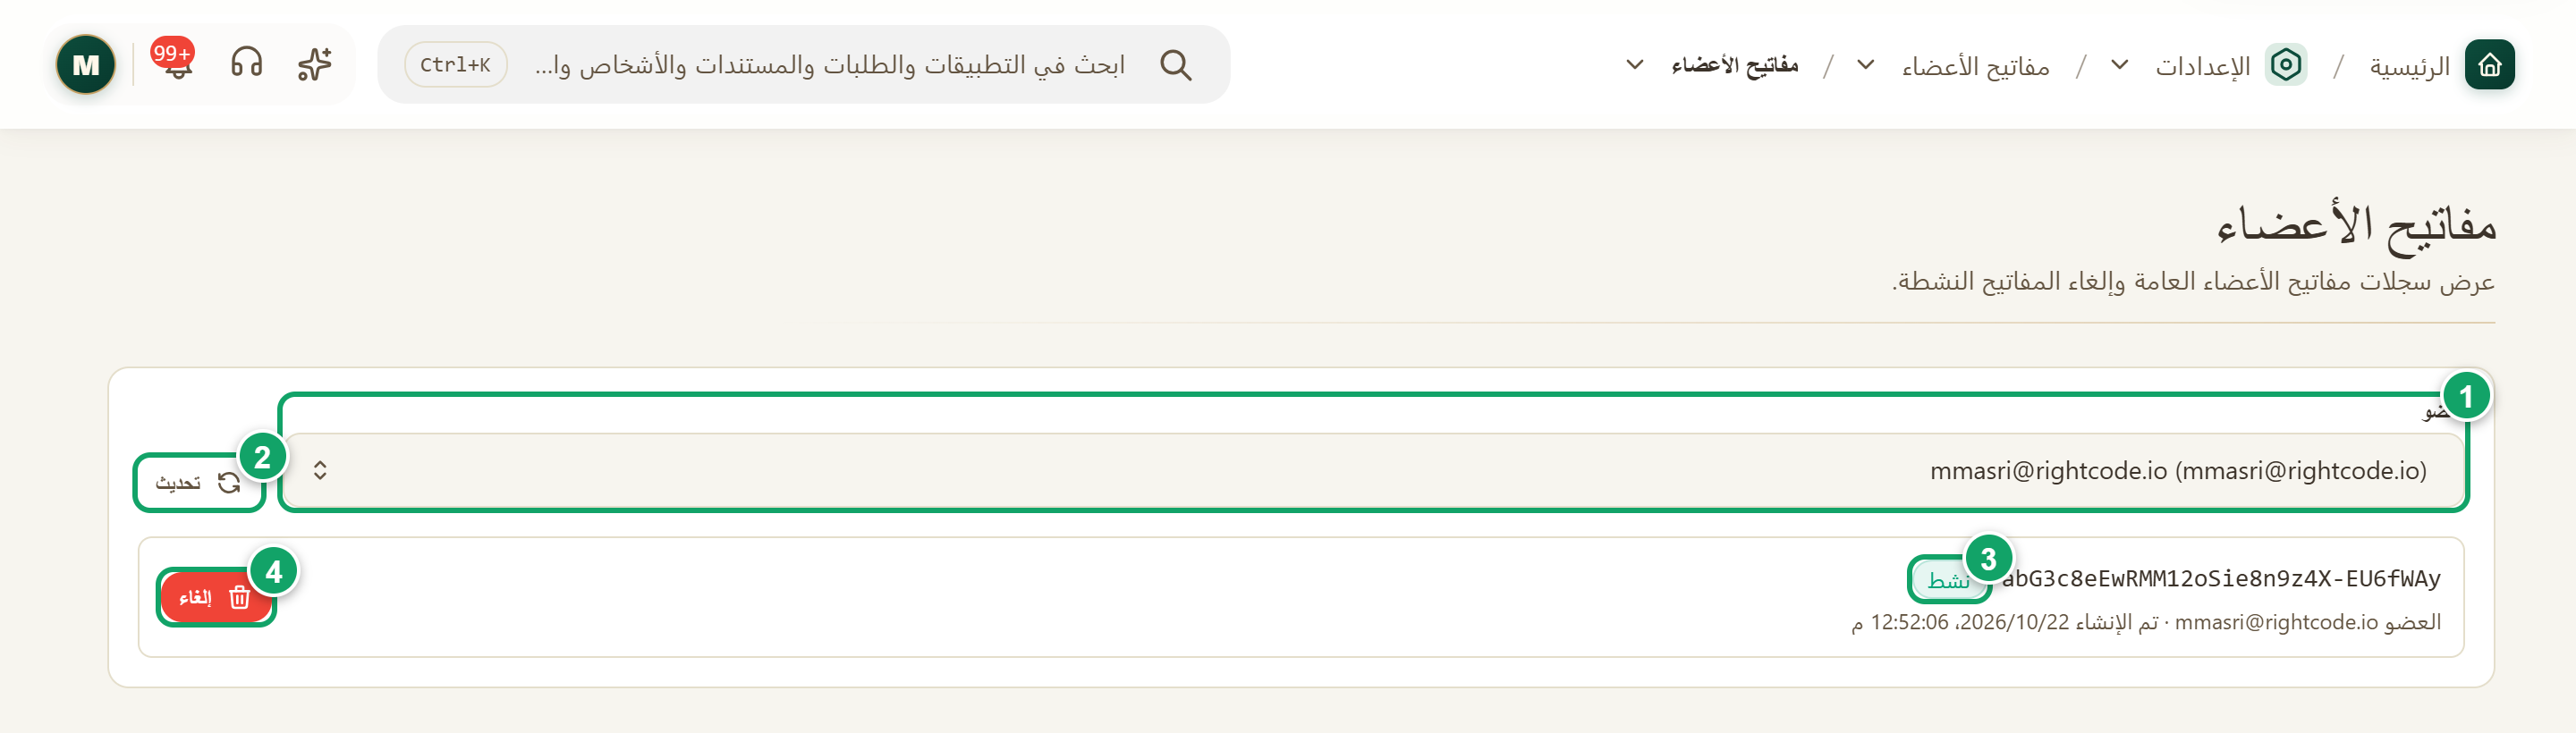
\includegraphics[width=0.95\linewidth,height=0.72\textheight,keepaspectratio]{figures/screens/ch08-member-keys-ar.png}
\caption{مفاتيح عضو في صفحة «مفاتيح الأعضاء»}
\label{fig:settings-member-keys-screen}
\shotnote{تبدأ الصفحة فارغة برسالة «لا توجد مفاتيح أعضاء مسجلة.» حتى تختار عضواً، ثم تعرض مفاتيحه النشطة فقط بمعرّف كل مفتاح وتاريخ إنشائه. والمعرّف رقم تعريف عام وليس المفتاح نفسه، والمفتاح المعروض يخص حساب اختبار. ① «العضو». ② «تحديث». ③ حالة المفتاح. ④ «إلغاء»: يوقف المفتاح ويخرجه من هذه القائمة.}
\end{figure}

\begin{table}[H]
\centering
\caption{ماذا تعني حالة المفتاح؟}
\label{tab:settings-member-keys-status}
\begin{tabularx}{\linewidth}{R{4.2cm} Y}
\rcHeaderRow
\thh{الحالة} & \thh{ماذا تعني؟}\\
«نشط» & المفتاح صالح للتوقيع. وهذه هي الحالة الوحيدة التي تظهر في «مفاتيح الأعضاء».\\
«مستبدل» & سجّل العضو مفتاحاً أحدث فحلّ محل هذا المفتاح تلقائياً. يراه العضو في «إدارة التوقيع».\\
«ملغى» & أوقفه مسؤول أو عطّله العضو نفسه، ولا يمكن استخدامه في توقيع جديد. يراه العضو في «إدارة التوقيع».\\
\end{tabularx}
\end{table}

\begin{enumerate}
\item اختر من «العضو» الشخص المطلوب، وتأكد من اسمه وبريده؛ فقد تتشابه الأسماء.
\item راجع المفتاح النشط، واضغط «تحديث» إذا كان العضو قد سجل مفتاحاً للتو.
\item لإيقاف مفتاح، اضغط «إلغاء» بجانبه ثم أكّد في نافذة «إلغاء مفتاح العضو».
\item إذا احتاج العضو إلى مفتاح جديد، فأصدر له رمز تسجيل من صفحة «إصدار رمز تسجيل» (\ref{sec:settings-feature-key-enrollments}).
\end{enumerate}

\textbf{تحقق:} يختفي المفتاح من القائمة، ويسجل «سجل التدقيق» حدث «تم إلغاء بيانات الاعتماد». لا يغيّر الإلغاء ما وُقّع سابقاً، ولا ينهي طلبات التوقيع المعلقة؛ فأعد توزيعها عبر مسارها.

\clearpage
\section{إصدار رمز تسجيل}
\label{sec:settings-feature-key-enrollments}

لا يستطيع العضو إنشاء مفتاح توقيع إلا برمز تسجيل يصدره له مسؤول. رمز التسجيل سلسلة أحرف قصيرة العمر: تنتهي صلاحيتها بعد 15 دقيقة، وتُستخدم مرة واحدة، ولا يستخدمها إلا العضو الذي صدرت باسمه. وبذلك يتأكد المسؤول من هوية العضو قبل التسجيل، بينما يولّد العضو مفتاحه بنفسه دون أن يراه أحد. استخدم الصفحة عند أول تسجيل، أو لاستبدال مفتاح مفقود. وهي تتطلب صلاحية تحديث الأعضاء.

\begin{rcnote}[مثال: شركة الأفق]
يتحقق مسؤول النظام من هوية سارة الخطيب، ويختارها عند ① ويضغط ②، ثم يسلمها الرمز مباشرة. تفتح سارة صفحة «إدارة التوقيع» فوراً وتكمل التسجيل قبل مرور 15 دقيقة.
\end{rcnote}

\begin{figure}[H]
\centering
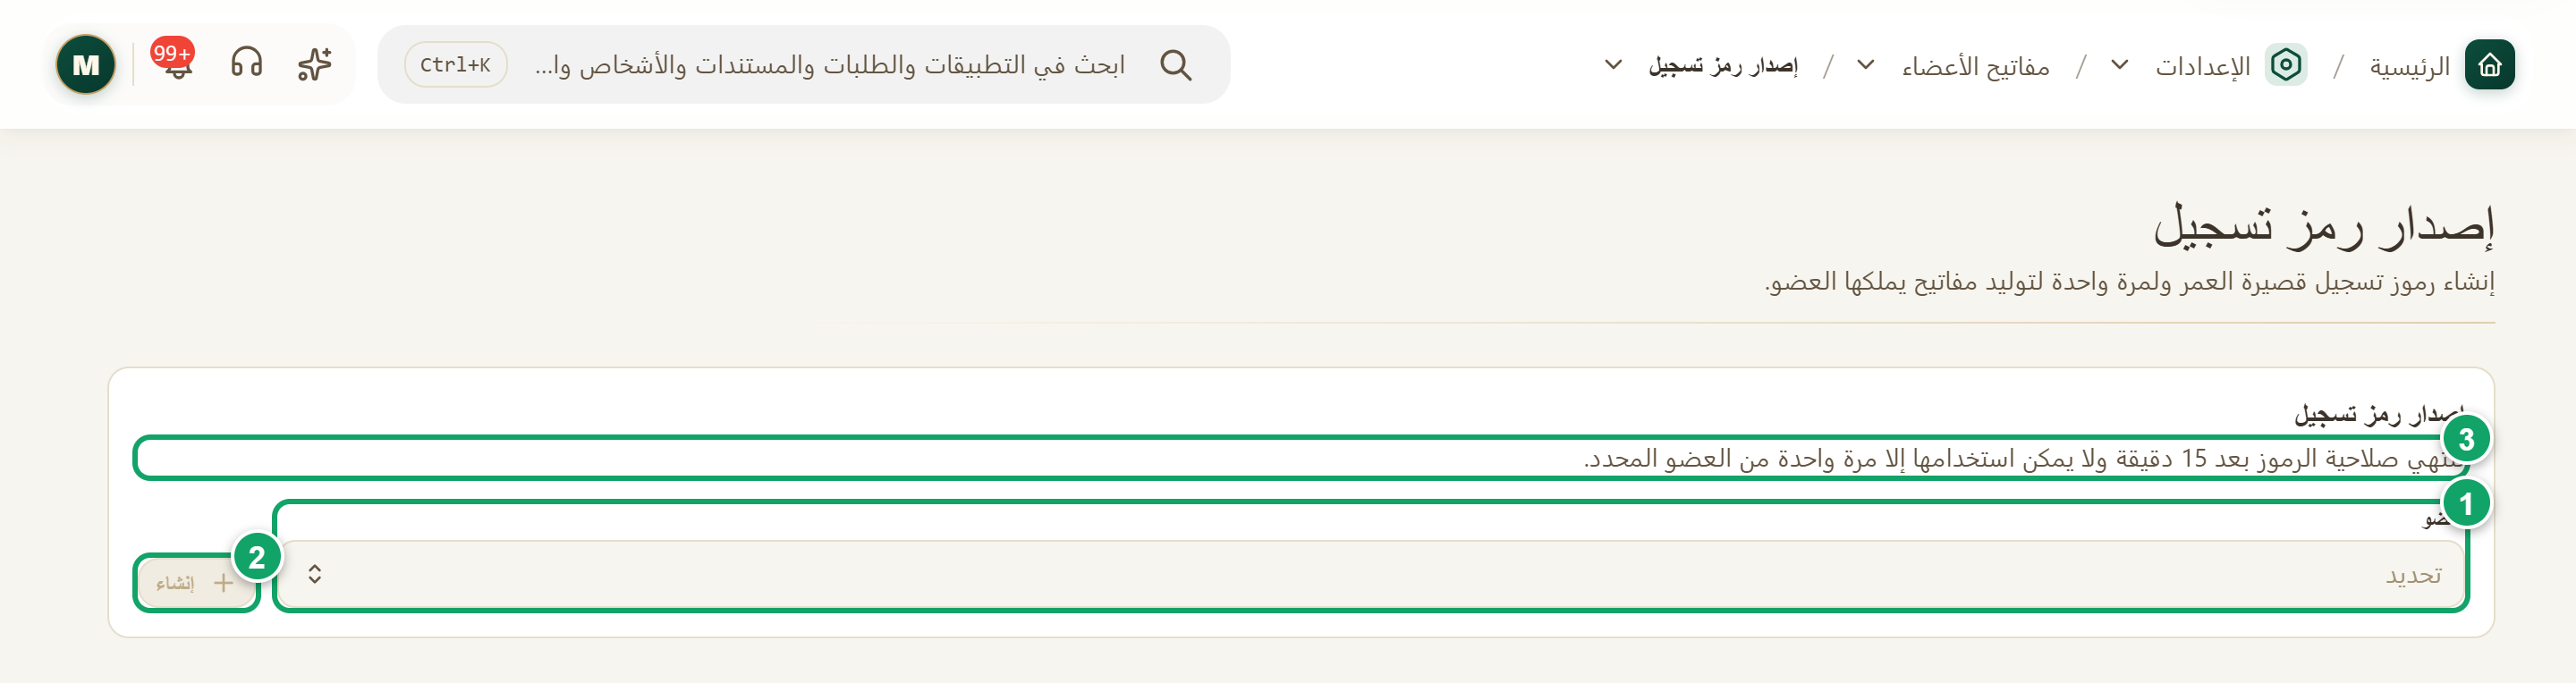
\includegraphics[width=0.95\linewidth,height=0.72\textheight,keepaspectratio]{figures/screens/ch08-key-enrollments-ar.png}
\caption{إصدار رمز تسجيل لعضو}
\label{fig:settings-key-enrollments-screen}
\shotnote{هذا نموذج قصير يربط الرمز بعضو واحد، ولا يتفعّل زر الإنشاء قبل اختياره. ولم يُصدر أي رمز عند التقاط الصورة، فهي لا تعرض قيمة حقيقية. ① «العضو». ② «إنشاء»: يعرض الرمز مرة واحدة مع زر «نسخ». ③ قاعدة الصلاحية: 15 دقيقة ومرة واحدة.}
\end{figure}

\begin{figure}[H]
\centering
\begin{tikzpicture}[node distance=0.5cm]
\node[stepBox] (a) {\RL{المسؤول يتحقق من هوية العضو}};
\node[stepBox,below=of a] (b) {\RL{المسؤول يصدر الرمز ويسلّمه بأمان}};
\node[stepBox,below=of b] (c) {\RL{العضو يدخل الرمز في «إدارة التوقيع»}};
\node[stepBox,below=of c] (d) {\RL{العضو يختار رمز \en{PIN} ويؤكده}};
\node[stepBox,below=of d] (e) {\RL{العضو يرسم توقيعه وينزّل الملف}};
\node[stepBox,below=of e] (f) {\RL{المسؤول يتأكد من حالة المفتاح «نشط»}};
\draw[flowsTo] (a) -- (b);
\draw[flowsTo] (b) -- (c);
\draw[flowsTo] (c) -- (d);
\draw[flowsTo] (d) -- (e);
\draw[flowsTo] (e) -- (f);
\end{tikzpicture}
\rclegend
\caption{رحلة تسجيل مفتاح العضو}
\label{fig:settings-key-journey-diagram}
\shotnote{يبين المخطط أين ينتقل العمل من المسؤول إلى العضو: يبدأ المسؤول الرحلة ويتحقق من نتيجتها، أما الخطوات الوسطى فيقوم بها العضو وحده. ولهذا لا يطّلع المسؤول على رمز \en{PIN} ولا على ملف المفتاح في أي مرحلة.}
\end{figure}

\begin{figure}[H]
\centering
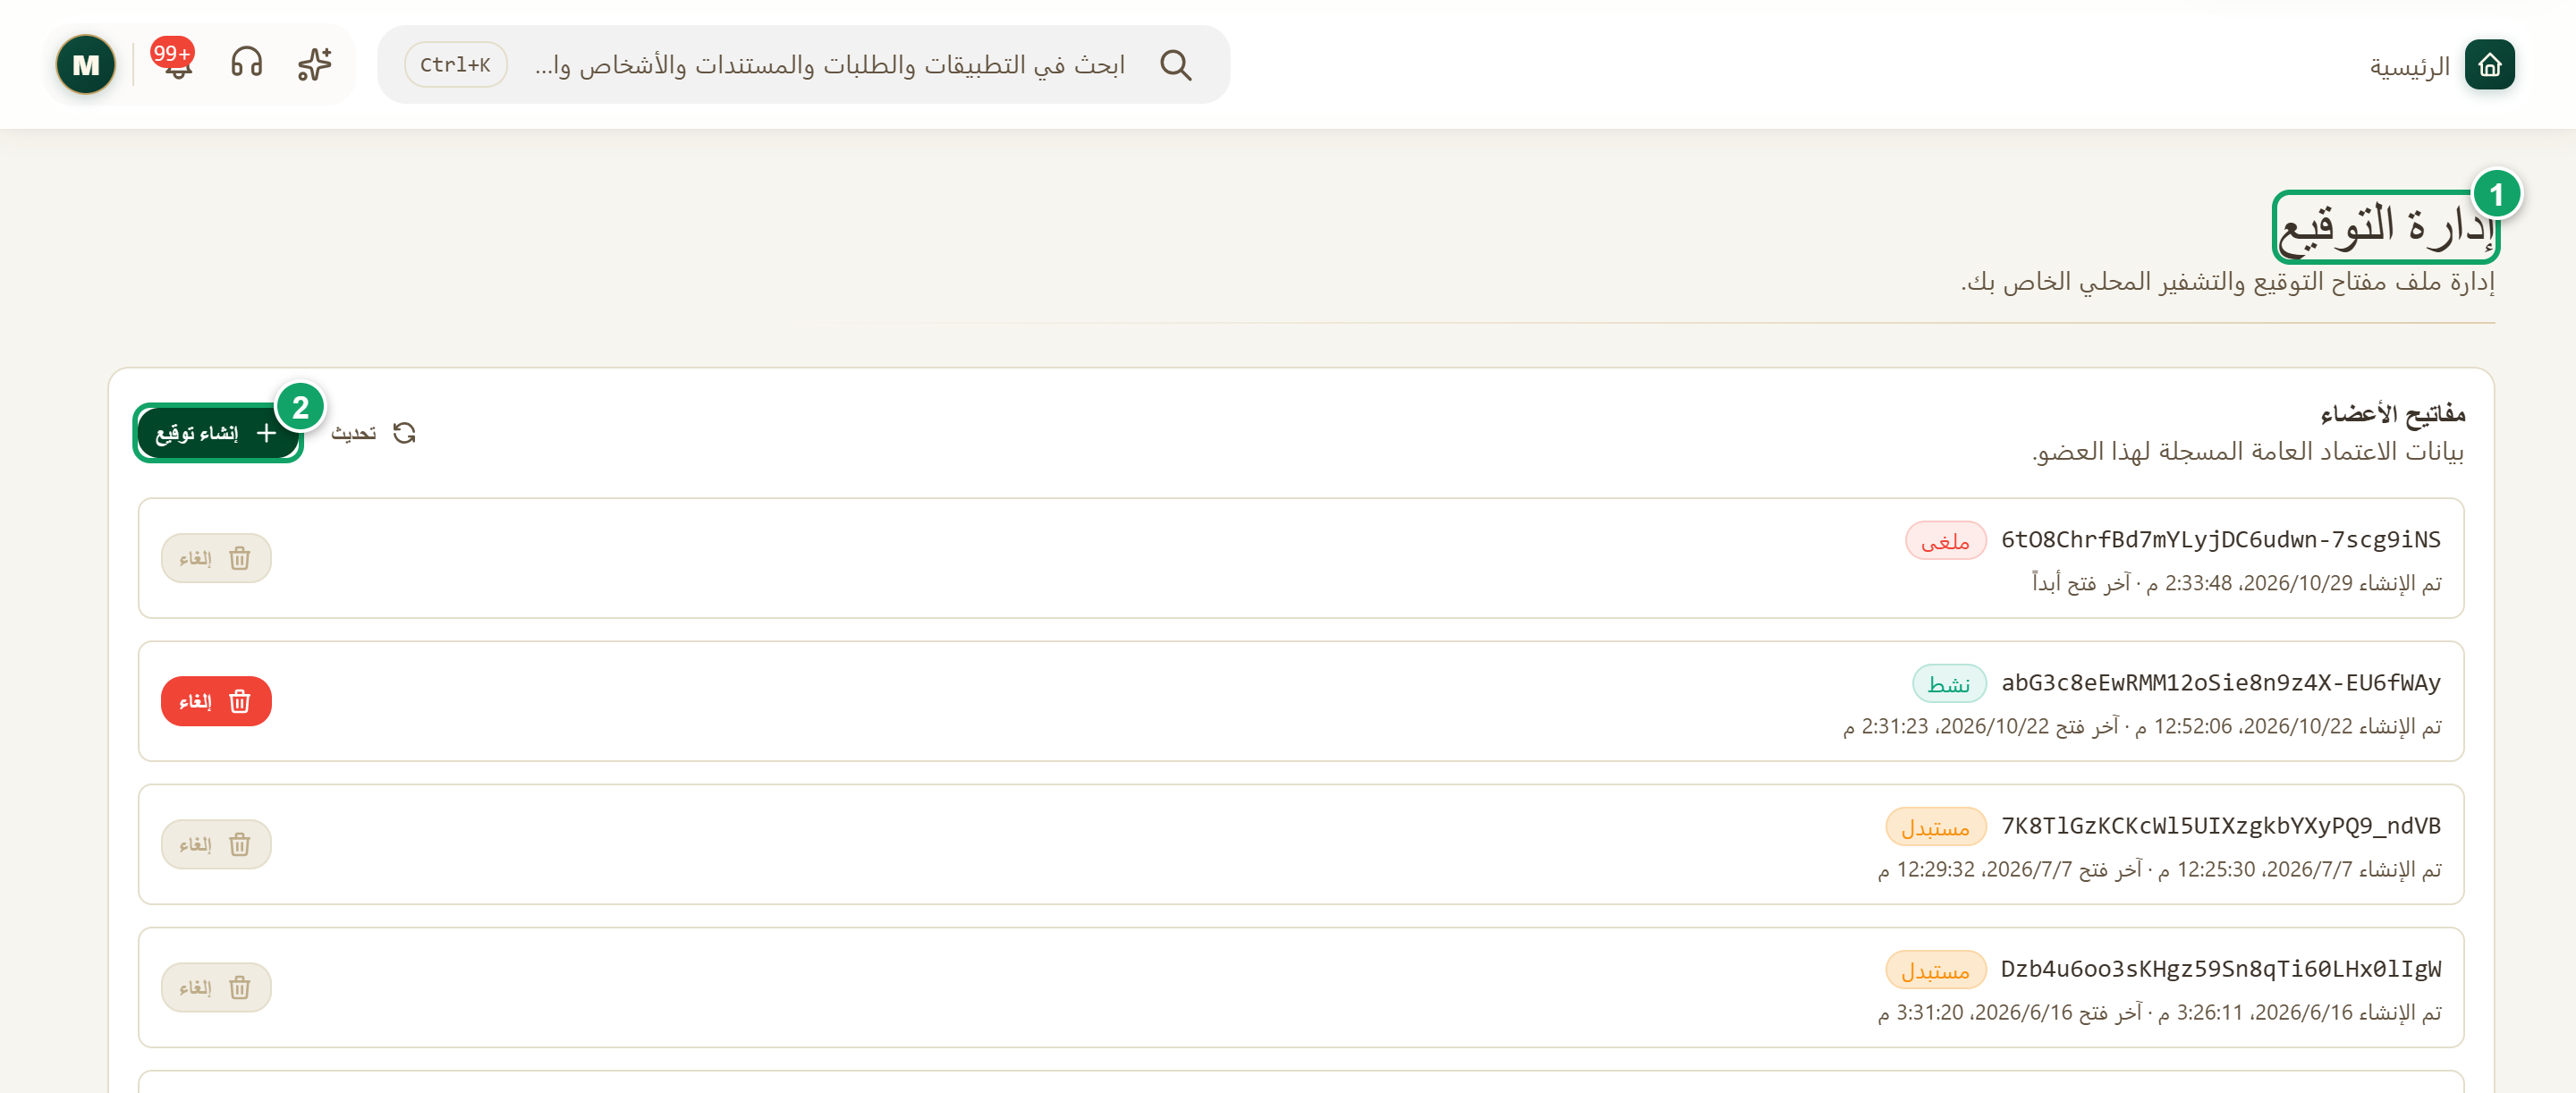
\includegraphics[width=0.95\linewidth,height=0.72\textheight,keepaspectratio]{figures/screens/ch08-key-member-ar.png}
\caption{صفحة «إدارة التوقيع» التي يكمل منها العضو التسجيل}
\label{fig:settings-key-member-screen}
\shotnote{هذه صفحة العضو الشخصية، وليست من الإعدادات، وفيها يستخدم الرمز الذي تسلمه ويرى مفاتيحه بكل حالاتها. ويخرج منها بملف مفتاح يحفظه في مكان خاص؛ فلا يمكن استرداد المفتاح إذا ضاع الملف. والمفاتيح المعروضة تخص حساب اختبار. ① «إدارة التوقيع». ② «إنشاء توقيع»: يبدأ خطوات التسجيل الأربع.}
\end{figure}

\begin{table}[H]
\centering
\caption{ماذا يسجل العضو في خطوات «إنشاء توقيع»؟}
\label{tab:settings-key-enrollments-fields}
\begin{tabularx}{\linewidth}{R{4.2cm} Y}
\rcHeaderRow
\thh{الخطوة} & \thh{ما الذي يسجله فيها؟}\\
«رمز التسجيل» & الرمز الذي سلمه المسؤول.\\
«إعداد رمز \en{PIN}» & ستة أرقام، بلا تكرار لرقم واحد ولا أرقام متسلسلة ولا نمط مكرر.\\
«تأكيد رمز \en{PIN}» & الأرقام نفسها مرة ثانية.\\
«رسم التوقيع» & يرسم توقيعه هنا، أو يضغط «الرسم على الهاتف» لفتح رابط صالح 5 دقائق، ثم يضغط «إنشاء وتنزيل».\\
\end{tabularx}
\end{table}

\begin{enumerate}
\item تأكد من هوية العضو، وجهّز طريقة آمنة لتسليم الرمز قبل إصداره.
\item اختر العضو من «العضو» واضغط «إنشاء».
\item اضغط «نسخ» وسلّم الرمز إلى العضو مباشرة. لا تضعه في محادثة عامة أو تذكرة أو صورة شاشة.
\item اطلب من العضو فتح «إدارة التوقيع» والضغط على «إنشاء توقيع»، ثم إكمال الخطوات وحفظ الملف.
\end{enumerate}

\textbf{تحقق:} يظهر للعضو مفتاح جديد بحالة «نشط» في «مفاتيح الأعضاء»، ويسجل «سجل التدقيق» حدث «اكتمل التسجيل». وإذا كان للعضو مفتاح سابق نشط أصبح «مستبدل». وإذا انتهت صلاحية الرمز قبل الإكمال، فأصدر رمزاً جديداً.

\clearpage
\section{سجل التدقيق}
\label{sec:settings-feature-key-audit}

يحفظ سجل التدقيق ما جرى لمفاتيح عضو معين: من أصدر رمز التسجيل، ومتى فُتح المفتاح، وهل فشلت المحاولات، ومتى أُلغي. راجعه عند اكتمال تسجيل جديد، أو عند الشك في استخدام مفتاح، أو عند قفله مؤقتاً. وهو للقراءة فقط، ويتطلب صلاحية تحديث الأعضاء. ويعرض أحدث 100 حدث للعضو المختار.

\begin{rcnote}[مثال: شركة الأفق]
يشكو عمر حداد من تعذر فتح مفتاحه. يختاره مسؤول النظام عند ①، فيجد محاولات فاشلة تبعها قفل مؤقت، فيطلب منه الانتظار والتأكد من رمز \en{PIN} بدل إصدار مفتاح جديد.
\end{rcnote}

\begin{figure}[H]
\centering
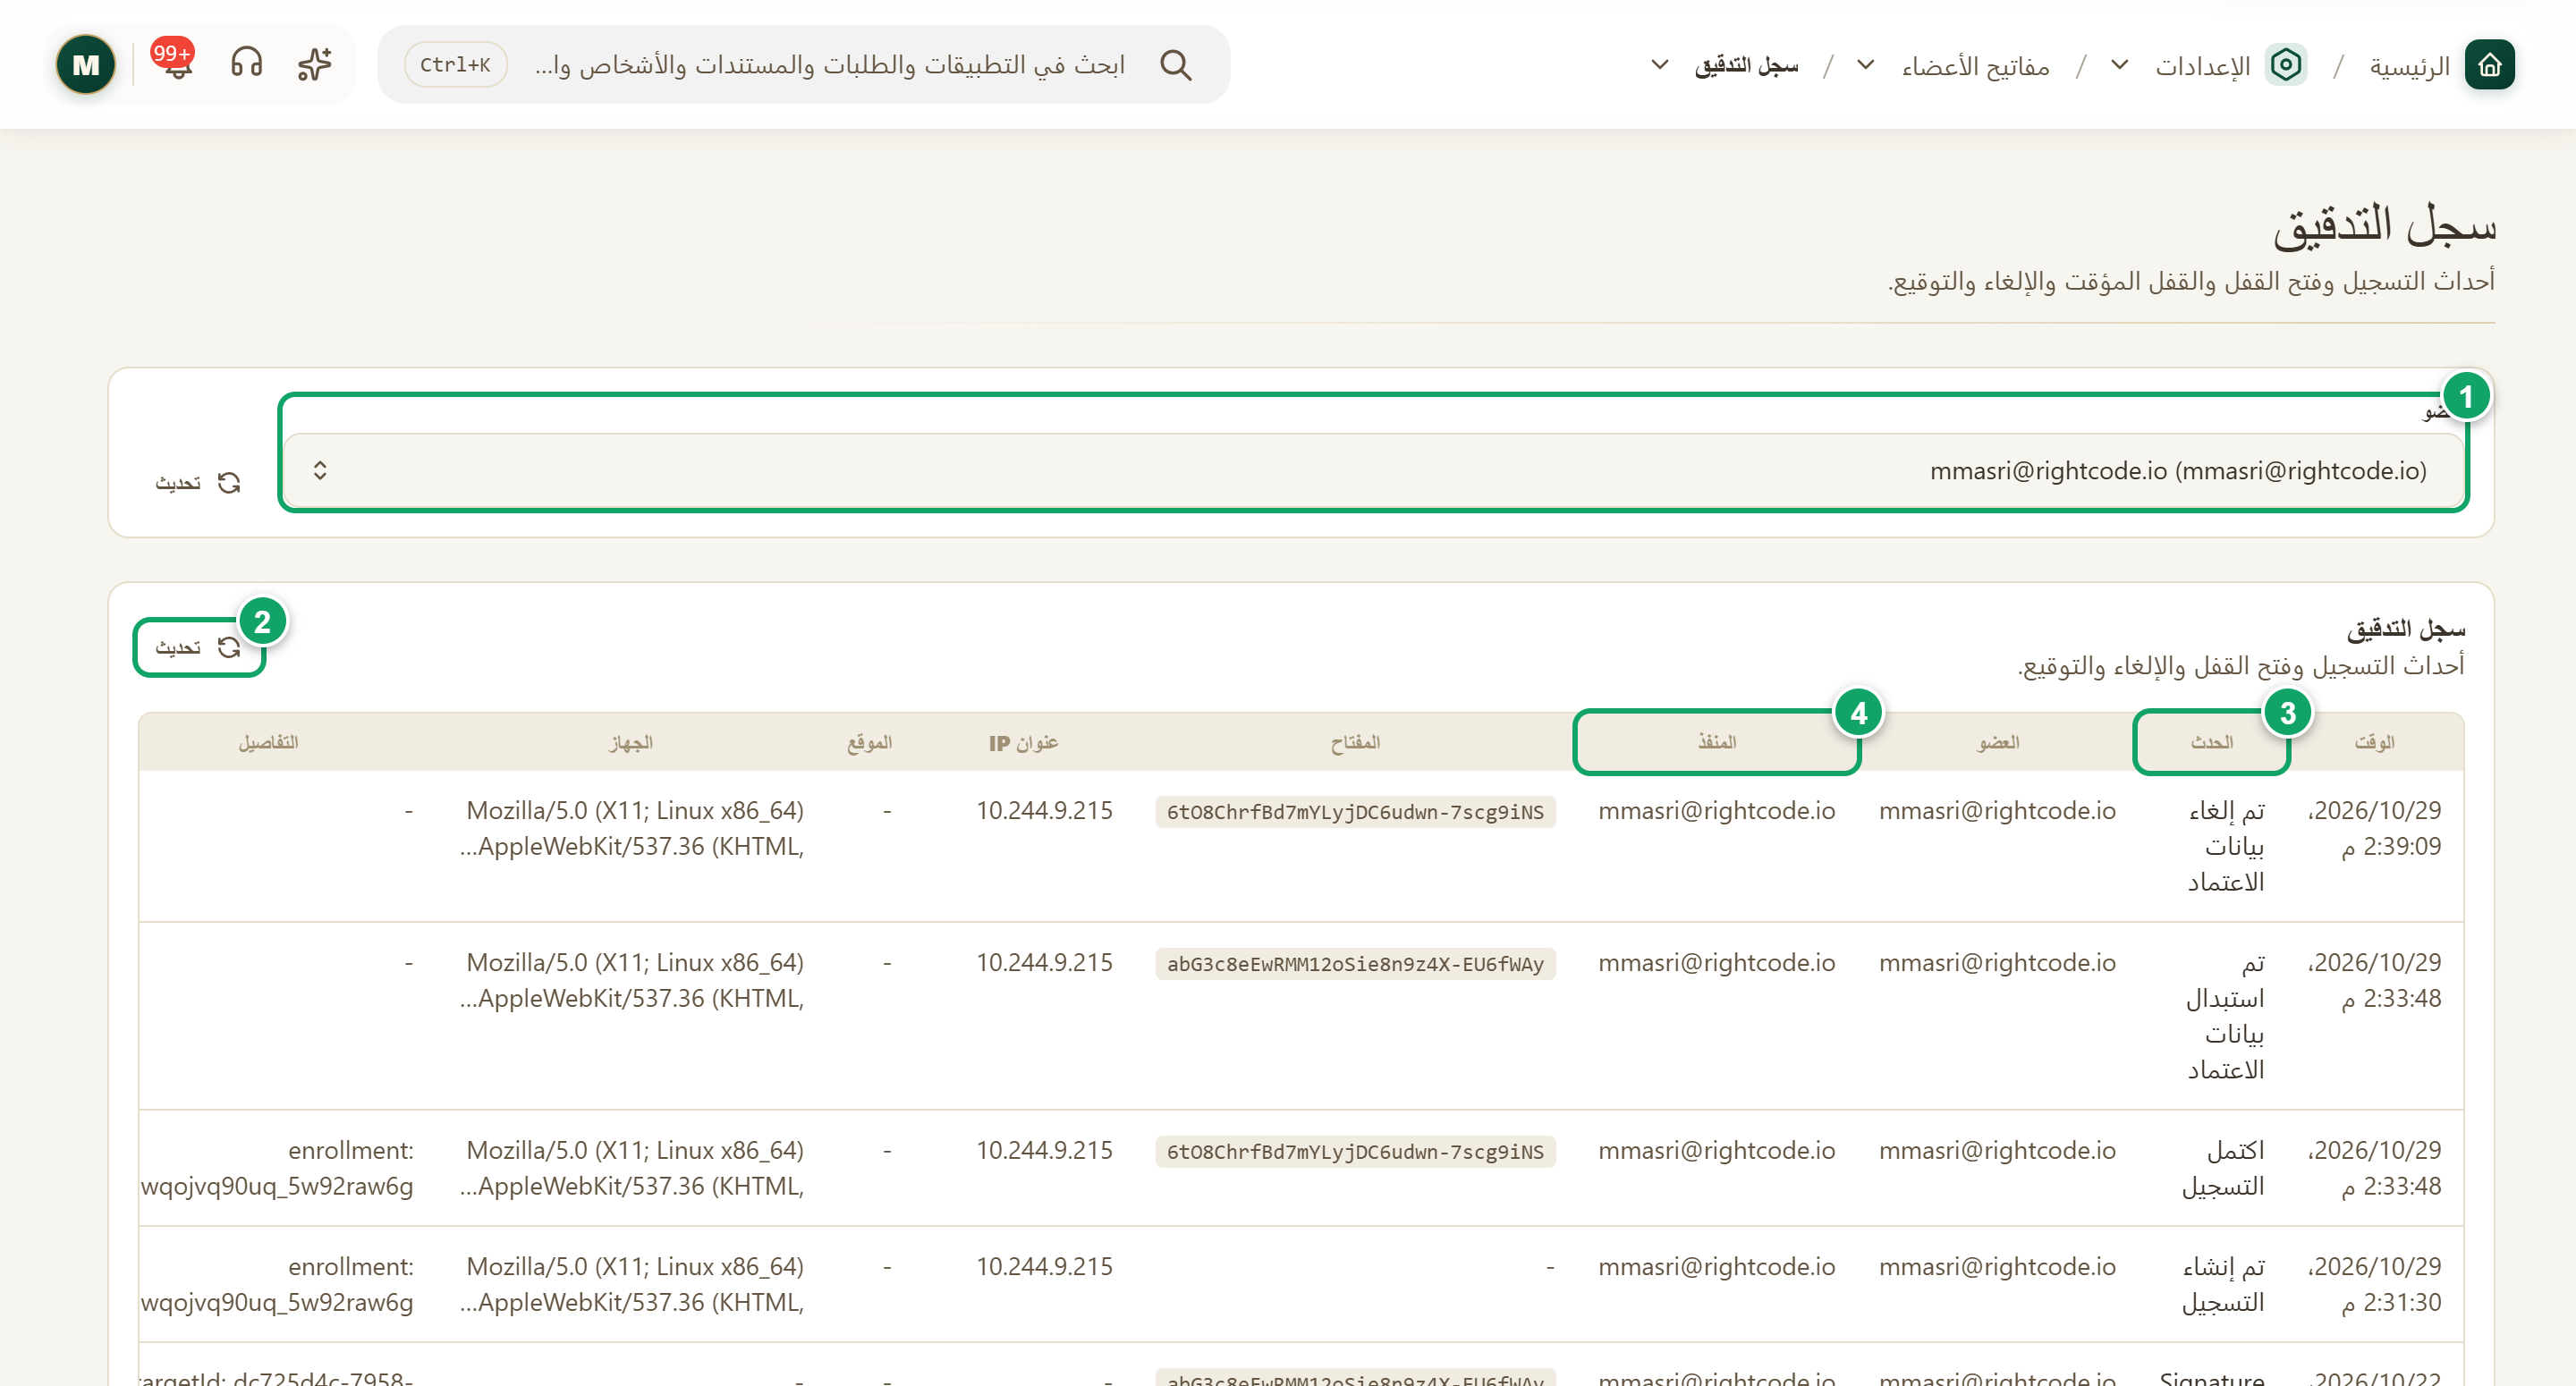
\includegraphics[width=0.95\linewidth,height=0.72\textheight,keepaspectratio]{figures/screens/ch08-key-audit-ar.png}
\caption{سجل تدقيق مفاتيح الأعضاء}
\label{fig:settings-key-audit-screen}
\shotnote{يبقى السجل فارغاً حتى تختار عضواً، ثم يعرض جدولاً من الأحدث إلى الأقدم فيه وقت الحدث ونوعه ومنفذه والمفتاح والجهاز. والأحداث المعروضة تخص حساب اختبار. ① «العضو». ② «تحديث». ③ «الحدث». ④ «المنفذ»: من قام بالإجراء، وقد يختلف عن العضو صاحب المفتاح.}
\end{figure}

\begin{table}[H]
\centering
\caption{ماذا تعني أبرز أحداث السجل؟}
\label{tab:settings-key-audit-events}
\begin{tabularx}{\linewidth}{R{4.2cm} Y}
\rcHeaderRow
\thh{الحدث} & \thh{ماذا يعني؟}\\
«تم إنشاء التسجيل» و«اكتمل التسجيل» & صدر رمز تسجيل، ثم أتم العضو إنشاء مفتاحه به.\\
«تم استبدال بيانات الاعتماد» و«تم إلغاء بيانات الاعتماد» & حلّ مفتاح جديد محل القديم، أو أوقف شخص المفتاح.\\
«بدأ فتح القفل» و«تم فتح القفل بنجاح» و«فشل فتح القفل» & محاولة استخدام المفتاح بملفه ورمز \en{PIN} ونتيجتها.\\
\en{Unlock Locked} & بعد خمس محاولات فاشلة يُقفل المفتاح 30 دقيقة. ويظهر هذا الحدث بالإنجليزية في الواجهة العربية أيضاً.\\
«تم إرسال توقيع الهاتف» & وصل رسم التوقيع من الهاتف عبر الرابط المؤقت.\\
\end{tabularx}
\end{table}

\begin{enumerate}
\item اختر العضو من «العضو».
\item اقرأ الأحداث من الأحدث، وانظر في «المنفذ» و«عنوان \en{IP}» و«الموقع» و«الجهاز».
\item اضغط «تحديث» لجلب ما استجد.
\end{enumerate}

\textbf{تحقق:} يظهر الحدث الذي تبحث عنه بوقته واسم منفذه. وإذا رأيت محاولات لا يعرفها العضو، فألغِ المفتاح من «مفاتيح الأعضاء» وأصدر له رمزاً جديداً بعد التأكد من هويته.

\clearpage
\section{الواجهة البرمجية والتكاملات}
\label{sec:settings-feature-api}

الواجهة البرمجية باب تتصل منه أنظمة أخرى ببيانات المؤسسة دون تدخل شخص، مثل نظام مالي يقرأ السجلات كل ليلة. ويدخل النظام الخارجي برمز \en{API}، وهو سلسلة سرية طويلة تحدد من يعمل هذا النظام باسمه وما يحق له. تجمع هذه الصفحة الرموز ومن يملكها ونشاطها والقواعد العامة لها. يرى كل عضو تبويب «الرموز» ورموزه الخاصة، أما إنشاء الرموز وبقية التبويبات فتظهر بحسب صلاحيات الدور، مثل «إنشاء رموز \en{API}» و«إدارة سياسة \en{API}».

\begin{rcnote}[مثال: شركة الأفق]
يطلب قسم المالية في شركة الأفق ربط نظامه بكيان. لا يربطه مسؤول النظام برمز عمر حداد الشخصي، بل يضغط «حساب خدمة جديد» في تبويب «حسابات الخدمة»، ثم ينشئ للحساب رمزاً بالقراءة فقط، فيبقى التكامل عاملاً إذا غادر أي موظف.
\end{rcnote}

\begin{figure}[H]
\centering
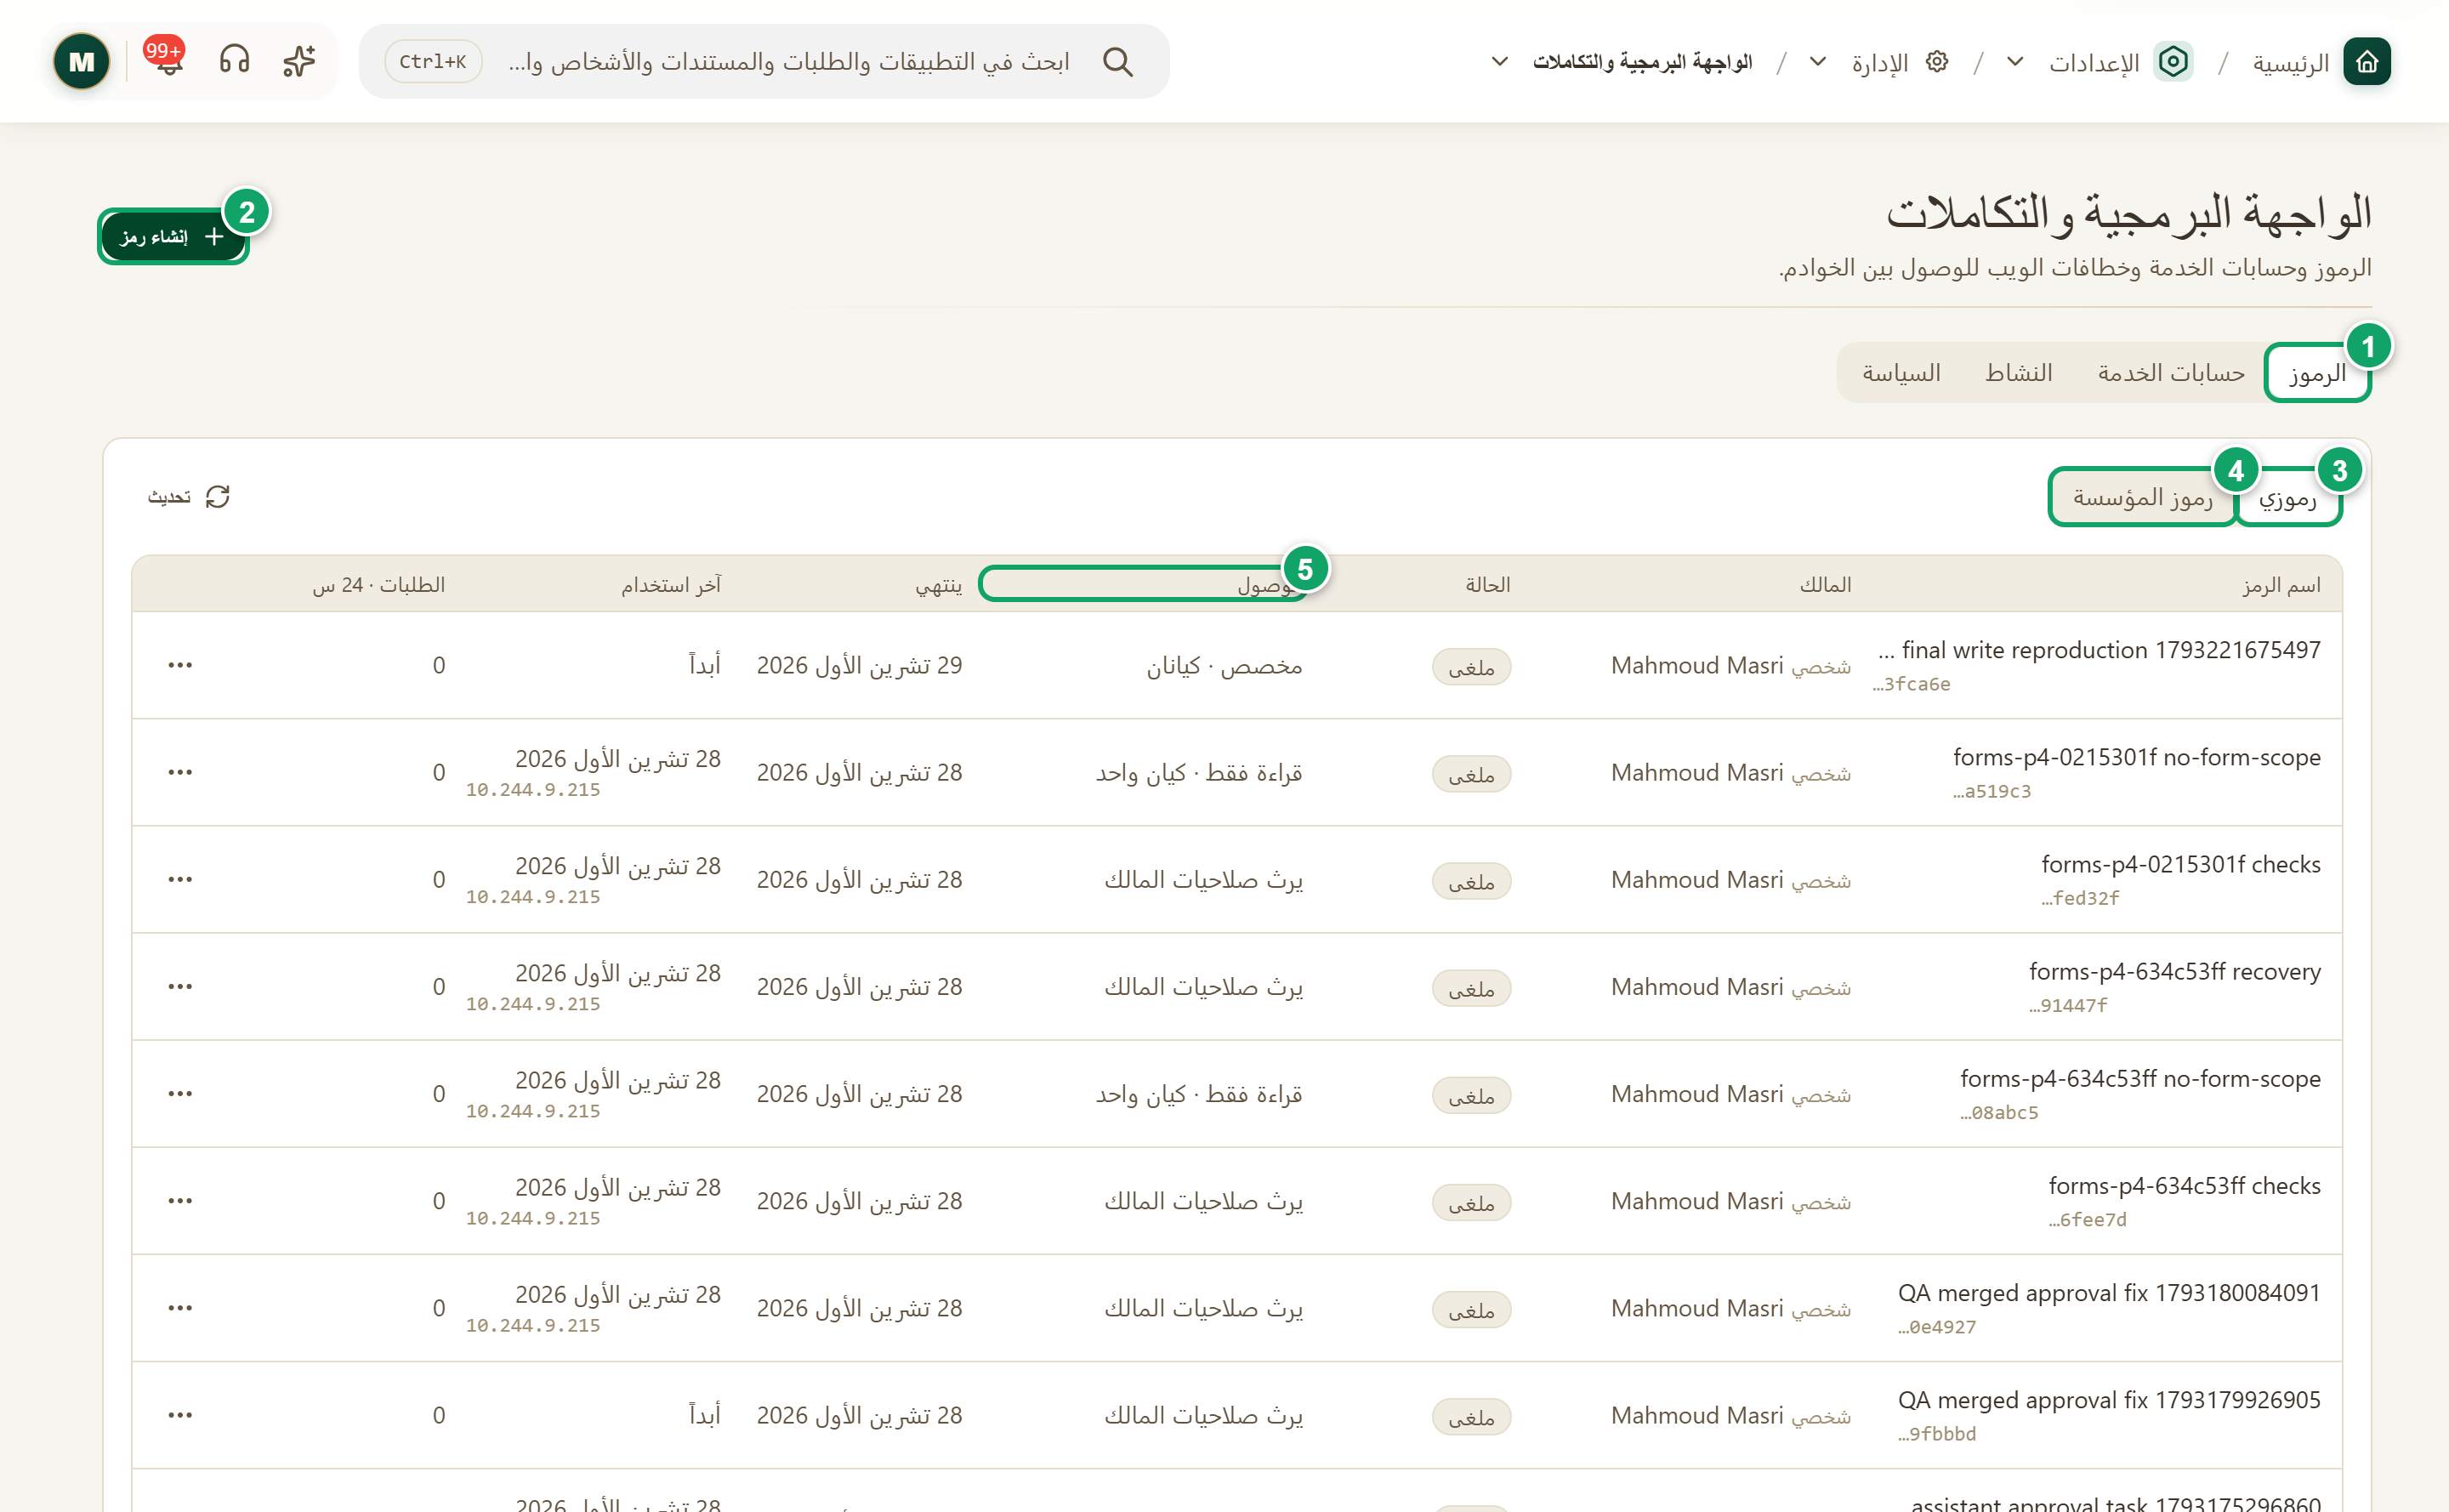
\includegraphics[width=0.95\linewidth,height=0.72\textheight,keepaspectratio]{figures/screens/ch08-api-tokens-ar.png}
\caption{تبويب «الرموز»}
\label{fig:settings-api-tokens-screen}
\shotnote{يعرض الجدول كل رمز بمالكه وحالته وصلاحياته وتاريخ انتهائه وآخر استخدامه. ولا يظهر الرمز نفسه أبداً، بل نهايته المختصرة فقط، والرموز المعروضة رموز اختبارية ملغاة. ① «الرموز». ② «إنشاء رمز». ③ «رموزي». ④ «رموز المؤسسة»: يظهر لمن يملك صلاحية الاطلاع عليها. ⑤ «الوصول»: ما يستطيعه الرمز باختصار.}
\end{figure}

\begin{figure}[H]
\centering
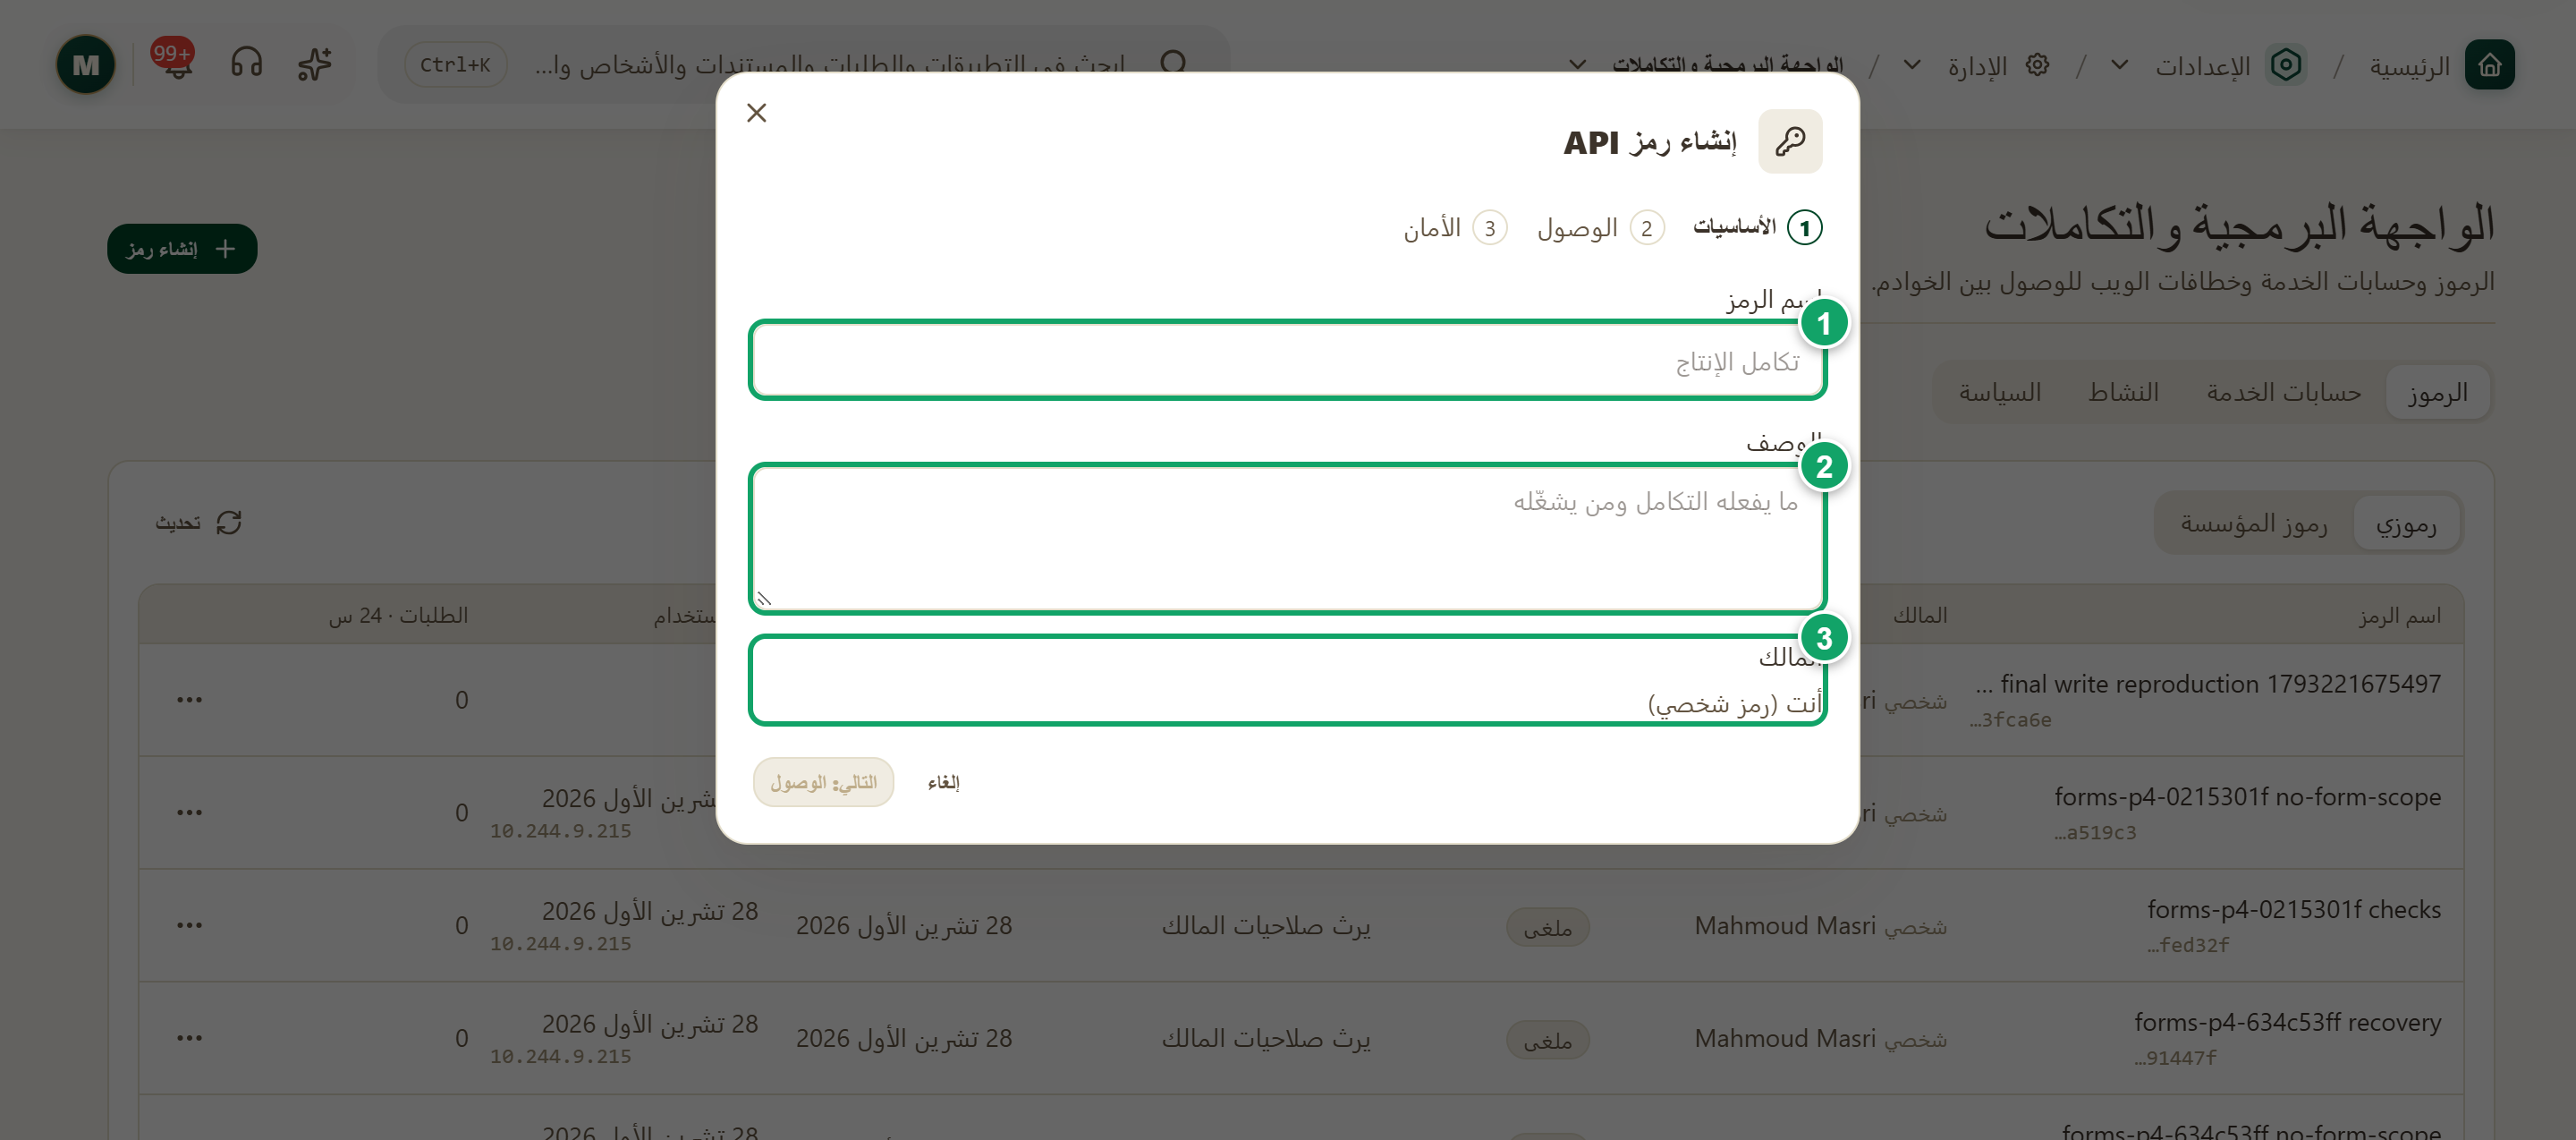
\includegraphics[width=0.95\linewidth,height=0.72\textheight,keepaspectratio]{figures/screens/ch08-api-create-ar.png}
\caption{نافذة إنشاء الرمز: خطوة «الأساسيات»}
\label{fig:settings-api-create-screen}
\shotnote{يمر إنشاء الرمز بثلاث خطوات: «الأساسيات» و«الوصول» و«الأمان». وقد فُتحت النافذة للقراءة ثم أُغلقت دون إنشاء رمز. ① «اسم الرمز»: اكتب اسماً يدل على النظام والغرض. ② «الوصف». ③ «المالك»: أنت لرمز شخصي، أو حساب خدمة تديره.}
\end{figure}

\begin{table}[H]
\centering
\caption{ماذا تسجل عند إنشاء الرمز؟}
\label{tab:settings-api-token-fields}
\begin{tabularx}{\linewidth}{R{4.2cm} Y}
\rcHeaderRow
\thh{الخطوة} & \thh{ما الذي تسجله فيها؟}\\
«الأساسيات» & «اسم الرمز» و«الوصف» و«المالك».\\
«الوصول» & «كل ما يستطيع المالك فعله»، أو «قراءة فقط»، أو «اختيار الكيانات والإجراءات». لا يتجاوز الرمز صلاحيات مالكه أبداً، والخيار الأخير هو الأضيق.\\
«الأمان» & تاريخ الانتهاء ضمن الحد الذي تسمح به السياسة، و«قائمة عناوين \en{IP} المسموح بها» إذا أردت قصر الرمز على شبكات معينة.\\
\end{tabularx}
\end{table}

\begin{figure}[H]
\centering
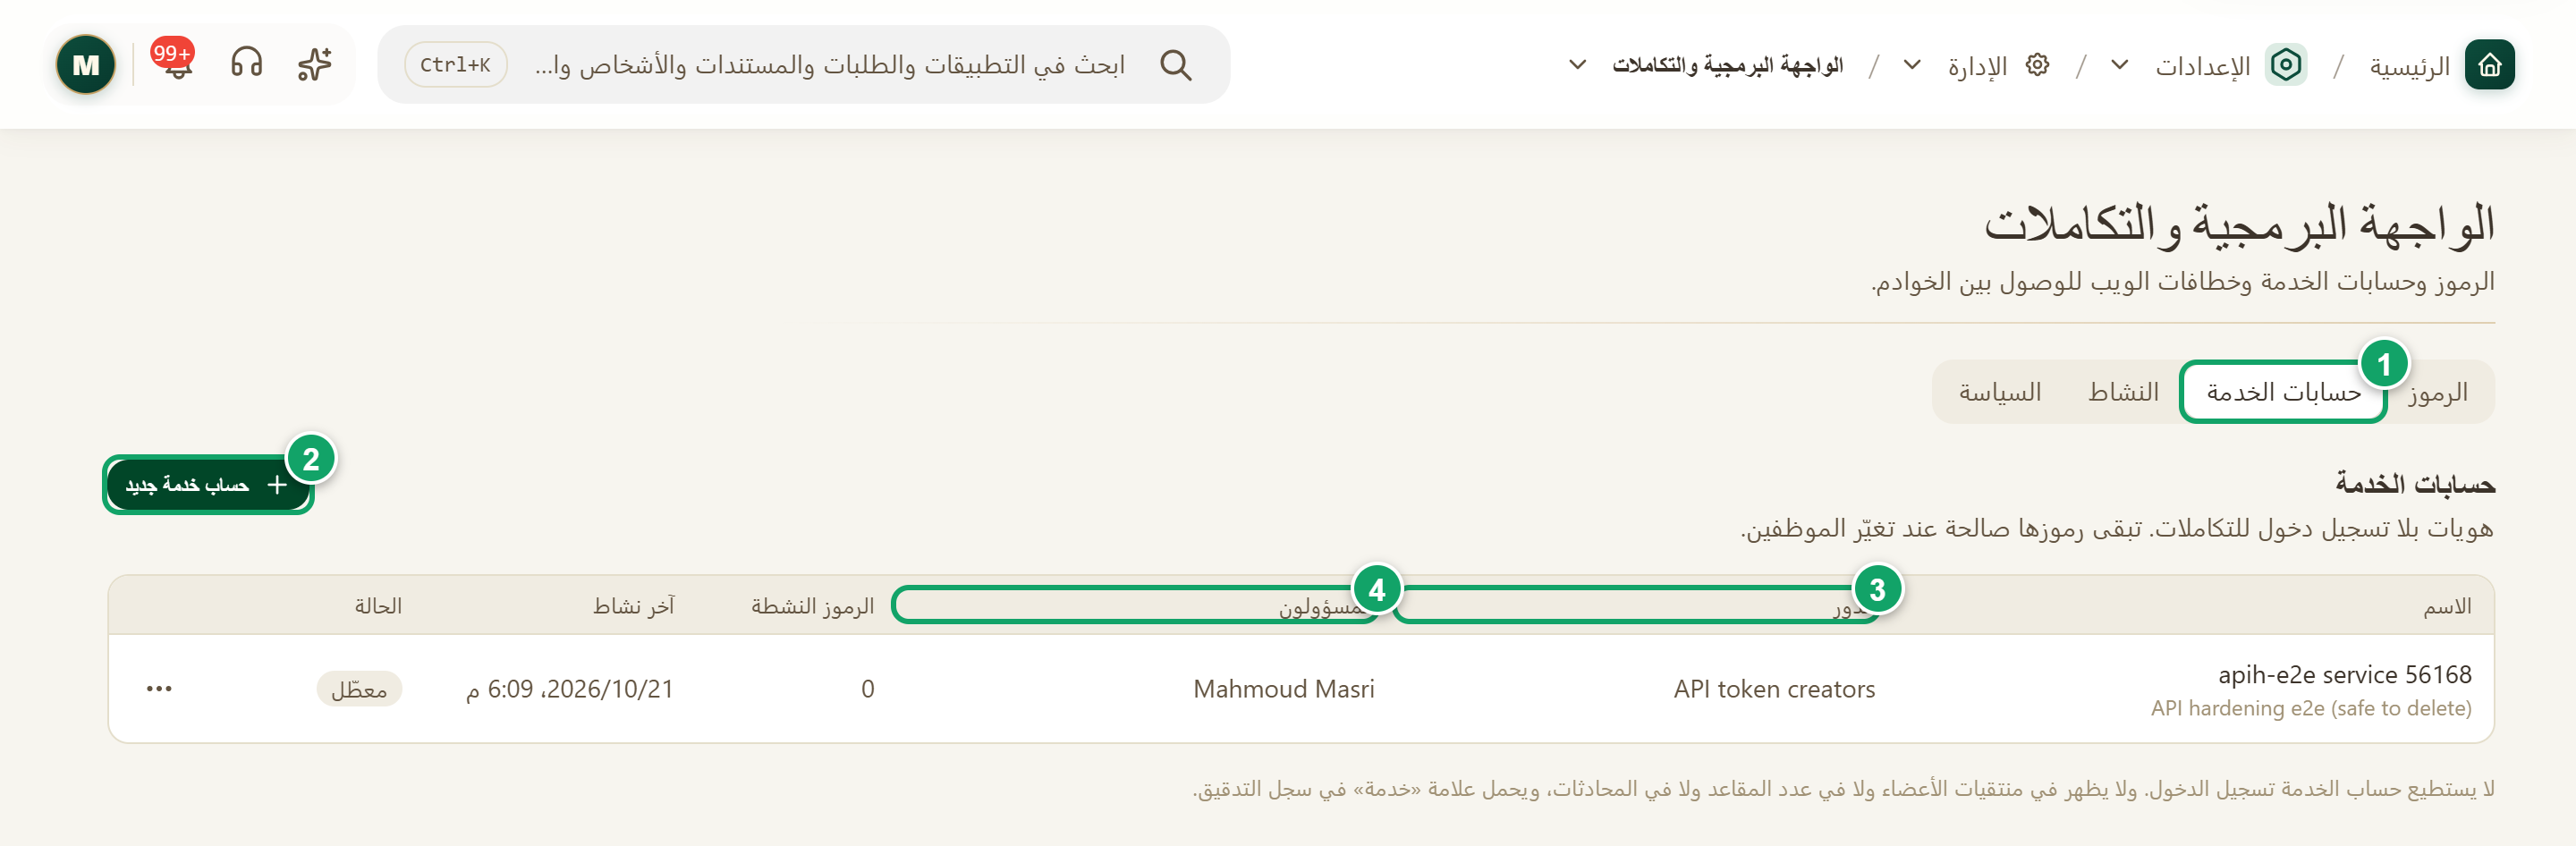
\includegraphics[width=0.95\linewidth,height=0.72\textheight,keepaspectratio]{figures/screens/ch08-api-service-accounts-ar.png}
\caption{تبويب «حسابات الخدمة»}
\label{fig:settings-api-service-accounts-screen}
\shotnote{حساب الخدمة هوية لتكامل واحد لا تسجّل الدخول، فلا يتوقف الرمز إذا غادر موظف. ولا يستطيع الحساب إلا ما يسمح به دوره، ولا يظهر في قوائم اختيار الأعضاء ولا يُحسب ضمن المقاعد. ① «حسابات الخدمة». ② «حساب خدمة جديد». ③ «الدور». ④ «المسؤولون»: من ينشئ رموز الحساب ويستبدلها ويتلقى تنبيهاتها.}
\end{figure}

\begin{figure}[H]
\centering
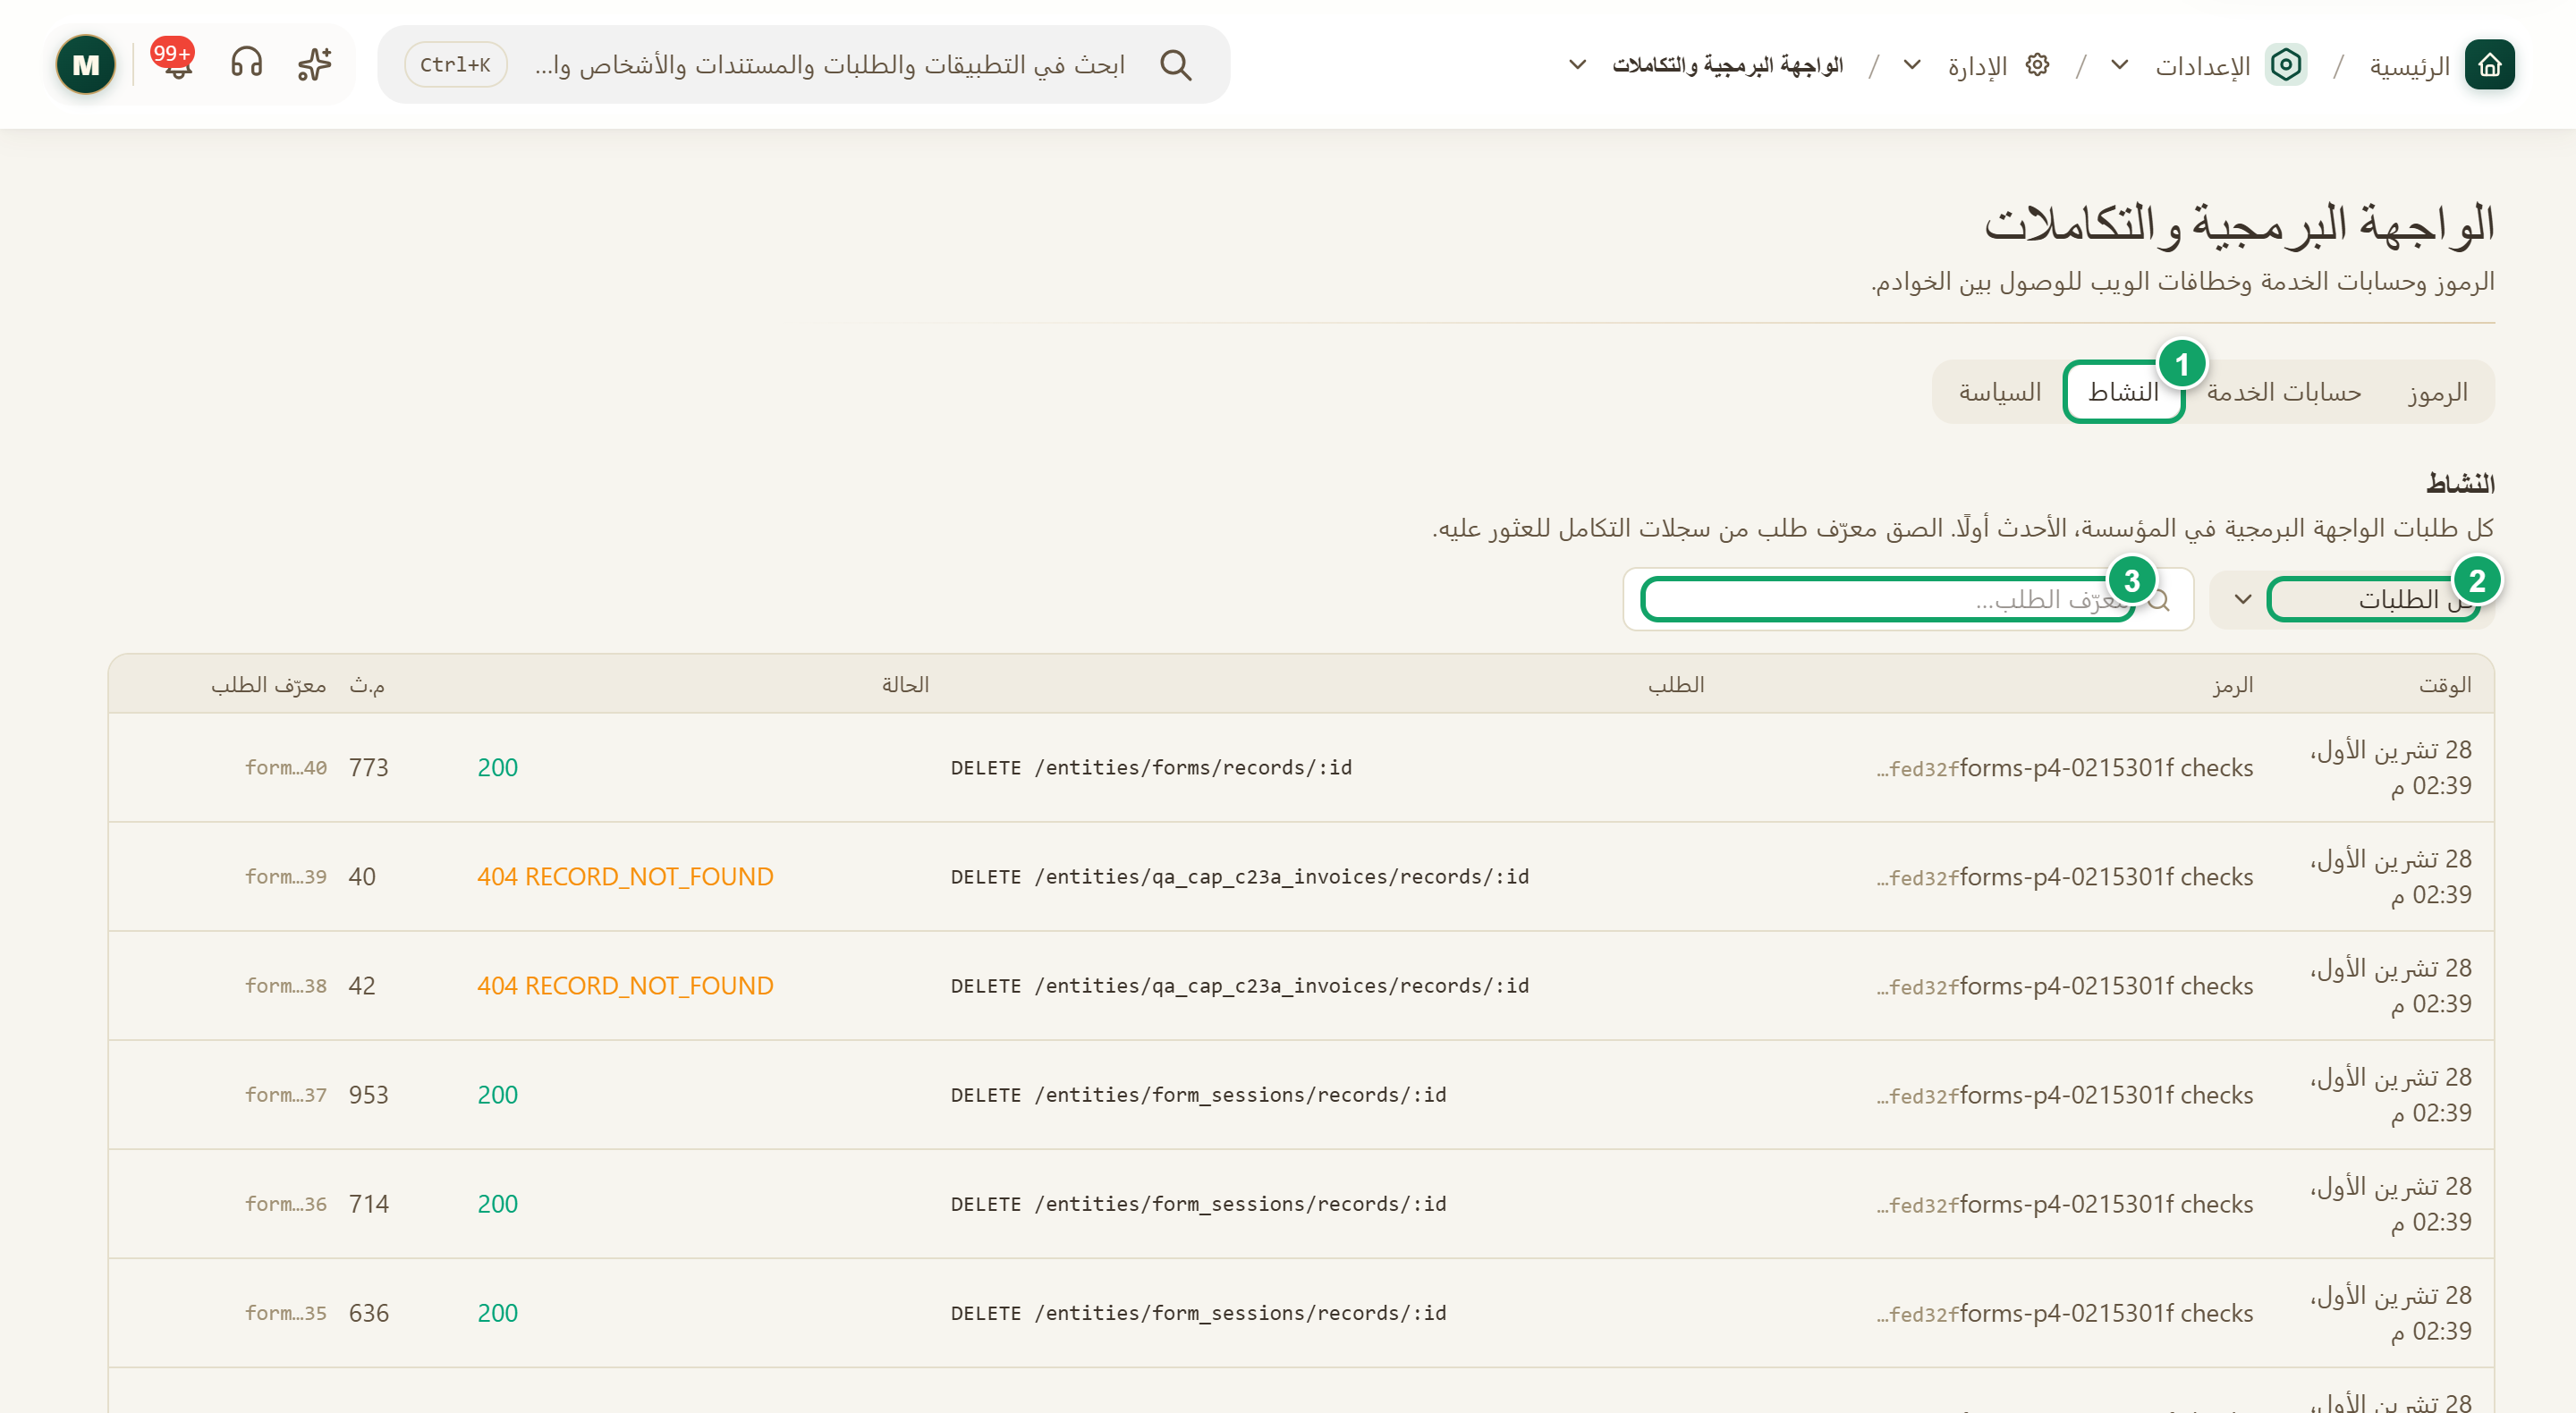
\includegraphics[width=0.95\linewidth,height=0.72\textheight,keepaspectratio]{figures/screens/ch08-api-activity-ar.png}
\caption{تبويب «النشاط»}
\label{fig:settings-api-activity-screen}
\shotnote{يعرض هذا التبويب طلبات الواجهة البرمجية في المؤسسة كلها من الأحدث إلى الأقدم، وهو نقطة البدء عند شكوى من تكامل متعطل. ولا تُحفظ محتويات الطلبات. ① «النشاط». ② مرشح الحالة: «كل الطلبات» أو «الأخطاء» أو «الناجحة». ③ «معرّف الطلب»: الصق المعرّف من سجلات التكامل للعثور على طلب بعينه.}
\end{figure}

\begin{figure}[H]
\centering
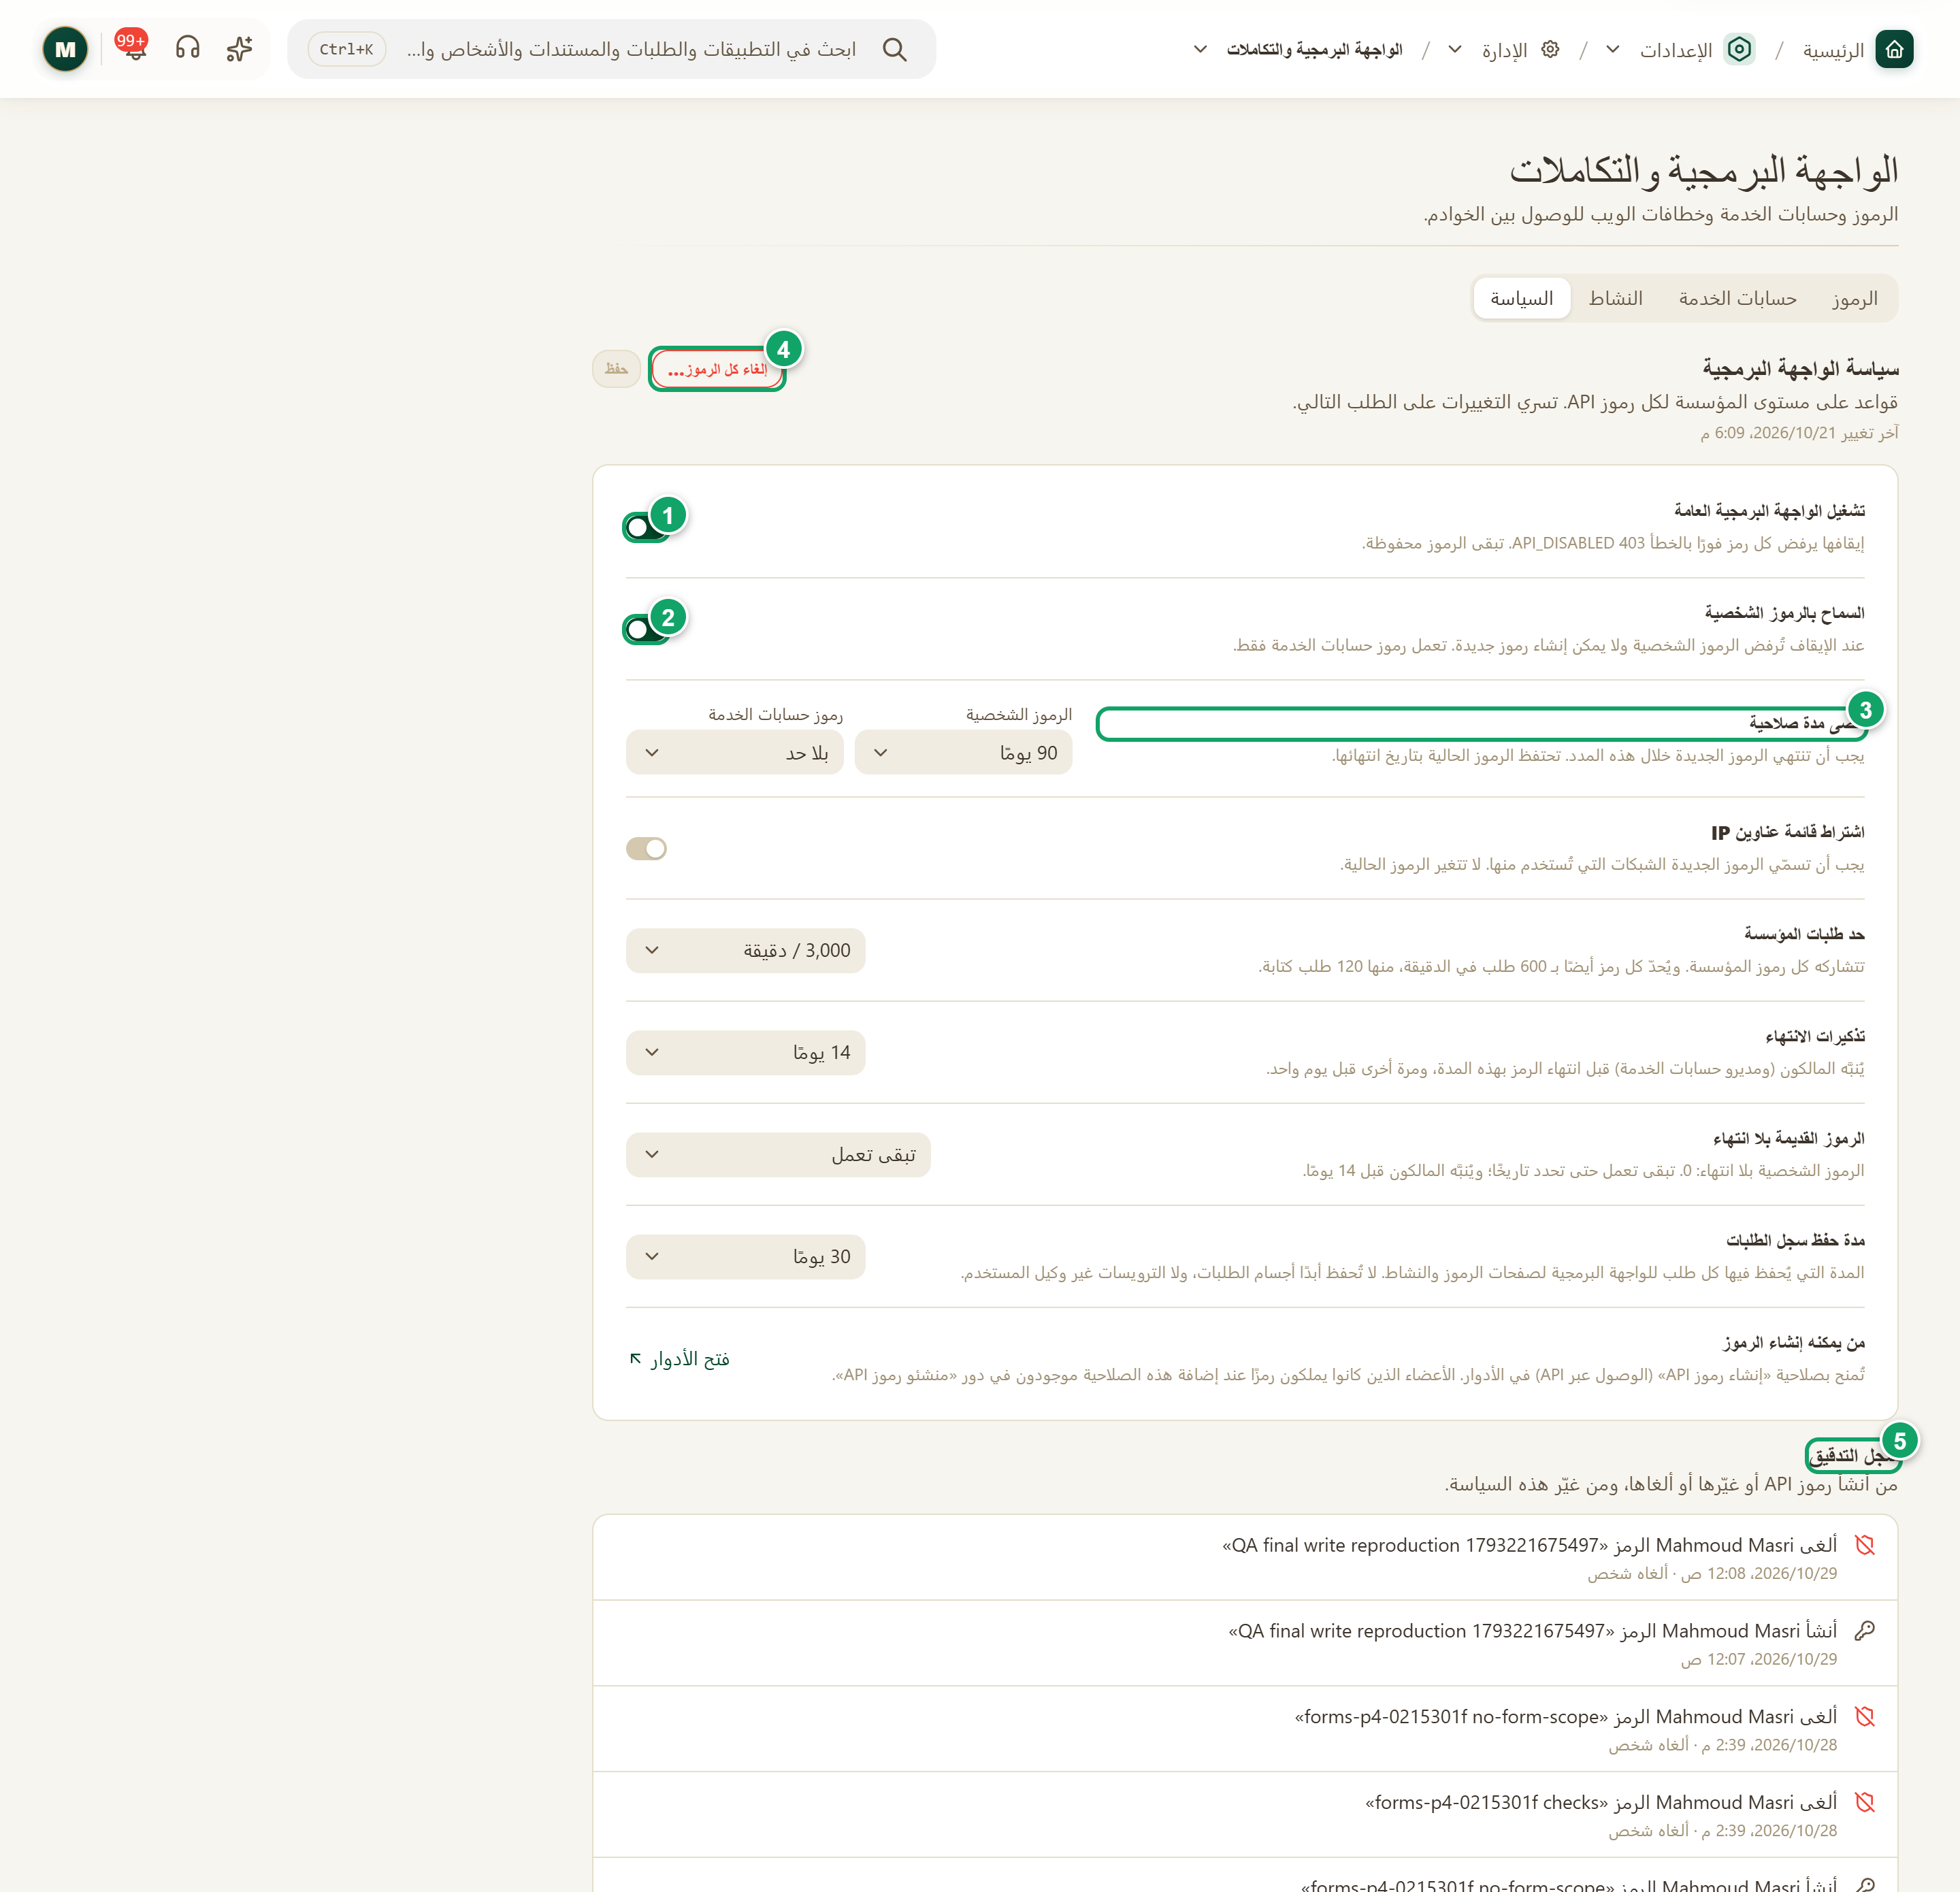
\includegraphics[width=0.95\linewidth,height=0.72\textheight,keepaspectratio]{figures/screens/ch08-api-policy-ar.png}
\caption{تبويب «السياسة» وسجل التدقيق}
\label{fig:settings-api-policy-screen}
\shotnote{تسري هذه القواعد على كل رموز المؤسسة من الطلب التالي للحفظ، لذلك غيّرها بحذر؛ فقد توقف تكاملات عاملة. وعُرضت الصفحة هنا للقراءة فقط. ① «تشغيل الواجهة البرمجية العامة»: إيقافها يرفض كل رمز فوراً وتبقى الرموز محفوظة. ② «السماح بالرموز الشخصية». ③ «أقصى مدة صلاحية»: تخص الرموز الجديدة. ④ «إلغاء كل الرموز…»: إجراء طوارئ لا يمكن التراجع عنه. ⑤ «سجل التدقيق»: من أنشأ الرموز أو غيّرها أو ألغاها، ومن غيّر السياسة.}
\end{figure}

\begin{table}[H]
\centering
\caption{ماذا تسجل في سياسة الواجهة البرمجية؟}
\label{tab:settings-api-policy-fields}
\begin{tabularx}{\linewidth}{R{4.2cm} Y}
\rcHeaderRow
\thh{الحقل} & \thh{ما الذي تسجله فيه؟}\\
«تشغيل الواجهة البرمجية العامة» & يوقف كل الرموز عند إطفائه، وتعود للعمل عند تشغيله.\\
«السماح بالرموز الشخصية» & عند الإيقاف تعمل رموز حسابات الخدمة فقط.\\
«أقصى مدة صلاحية» & حد «الرموز الشخصية» وحد «رموز حسابات الخدمة». لا تتأثر الرموز الحالية.\\
«اشتراط قائمة عناوين \en{IP}» & يلزم كل رمز جديد بتسمية الشبكات التي يُستخدم منها.\\
«حد طلبات المؤسسة» & عدد الطلبات في الدقيقة لكل رموز المؤسسة معاً.\\
«تذكيرات الانتهاء» & المدة التي يُنبَّه فيها المالكون قبل انتهاء الرمز، ثم مرة أخرى قبل يوم واحد.\\
«الرموز القديمة بلا انتهاء» & إبقاؤها عاملة، أو تحديد تاريخ توقفها.\\
«مدة حفظ سجل الطلبات» & مدة بقاء الطلبات في صفحات الرموز و«النشاط».\\
«من يمكنه إنشاء الرموز» & إشارة إلى صلاحية «إنشاء رموز \en{API}» في الأدوار، ومعها زر «فتح الأدوار».\\
\end{tabularx}
\end{table}

\begin{enumerate}
\item لتكامل دائم، افتح «حسابات الخدمة» واضغط «حساب خدمة جديد»، واكتب «الاسم» واختر «الدور» و«المسؤولون»، ثم اضغط «إنشاء».
\item افتح «الرموز» واضغط «إنشاء رمز»، وأكمل «الأساسيات» و«الوصول» و«الأمان»، واختر للتكامل الدائم حساب الخدمة في «المالك».
\item انسخ الرمز فور ظهوره إلى مكان آمن؛ فلن يظهر مرة أخرى. ثم أكّد حفظه واضغط «تم».
\item لاستبدال رمز قديم، افتح قائمة صفه واضغط «تدوير»، واختر مدة بقاء الرمز القديم صالحاً حتى 7 أيام، ثم حدّث التكامل.
\item لإيقاف رمز، افتح قائمة صفه واضغط «إلغاء»، ويتوقف الرمز فوراً.
\item لتغيير القواعد، افتح «السياسة»، وعدّل القيمة ثم اضغط «حفظ».
\end{enumerate}

\textbf{تحقق:} يظهر الرمز في الجدول بحالة «نشط»، ويتغير «آخر استخدام» بعد أول طلب، وتظهر الطلبات في «النشاط» وفي صفحة الرمز. ويسجل «سجل التدقيق» كل إنشاء أو إلغاء أو تغيير في السياسة. وإذا توقف تكامل، فابدأ من «النشاط»، ثم تحقق من حالة الرمز وتاريخ انتهائه ومن أن الواجهة البرمجية ما زالت مفعّلة.
